% This is part of Le Frido
% Copyright (c) 2006-2022
%   Laurent Claessens, Carlotta Donadello
% See the file fdl-1.3.txt for copying conditions.


%+++++++++++++++++++++++++++++++++++++++++++++++++++++++++++++++++++++++++++++++++++++++++++++++++++++++++++++++++++++++++++
\section{Règles de calcul}
%+++++++++++++++++++++++++++++++++++++++++++++++++++++++++++++++++++++++++++++++++++++++++++++++++++++++++++++++++++++++++++

D'abord une dérivée facile, qui sera utile pour démontrer la formule de dérivation d'un quotient.
\begin{lemma}
	Nous avons :
	\begin{equation}
		\left( \frac{1}{ x } \right)'=-\frac{1}{ x^2 }.
	\end{equation}
\end{lemma}

\begin{proof}
	En posant \( f(x)=1/x\), nous avons le calcul
	\begin{equation}
		\frac{ f(x+\epsilon)-f(x) }{ \epsilon }=\frac{ \frac{1}{ x+\epsilon }-\frac{1}{ x } }{ \epsilon }=\frac{ x-(x+\epsilon) }{ \epsilon x(x+\epsilon) }=\frac{ -1 }{ x(x+\epsilon) }.
	\end{equation}
	Nous trouvons le résultat en passant à la limite et en tenant compte de la proposition \ref{PROPooOUPNooTrClHw} sur la limite d'un quotient.
\end{proof}


\begin{proposition}[\cite{ooRCDWooONrayj,ooVNAOooAuQSse,ooOGGJooCGQgDO}]     \label{PROPooOUZOooEcYKxn}
	Nous avons les règles suivantes.
	\begin{enumerate}
		\item       \label{ITEMooTFNPooYngHnD}
		      Si \( f,g\colon \eR\to \eR\) sont dérivables en \( a\in \eR\), alors \( f+g\) est dérivable en \( a\) et
		      \begin{equation}
			      (f+g)'(a)=f'(a)+g'(a).
		      \end{equation}
		\item       \label{ITEMooIPLRooOZXqMg}
		      Si \( f\colon \eR\to \eR\) est dérivable en \( a\in \eR\) et si \( \lambda\in \eR\), alors \( (\lambda f)\) est dérivable en \( a\) et
		      \begin{equation}
			      (\lambda f)'(a)=\lambda f'(a).
		      \end{equation}
		\item   \label{ITEMooMQERooBCqnvS}
		      Si \( f,g\colon \eR\to \eR\) sont dérivables en \( a\in \eR\), alors \( fg\) est dérivable en \( a\) et
		      \begin{equation}
			      (fg)'(a)=f'(a)g(a)+f(a)g'(a).
		      \end{equation}
		      Cette formule est appelée \defe{règle de Leibnitz}{Leibnitz}.
		\item   \label{ITEMooLYZCooVUPTyh}
		      Soient deux intervalles \( I,J\) dans \( \eR\). Soient des fonctions \( f\colon I\to J\) et \( g\colon J\to \eR\). Soit encore \( a\in I\). SI \( f\) est dérivable en \( a\) et si \( g\) est dérivable en \( f(a)\), alors \( g\circ f\) est dérivable en \( a\) et
		      \begin{equation}
			      (g\circ f)'(a)= g'\big( f(a) \big)f'(a).
		      \end{equation}
		\item      \label{ITEMooMUNQooLiKffz}
		      Soient \( f,g\colon I\to \eR\) des fonction sur un intervalle ouvert \( I\). Soit \( a\in I\); supposons que \( g(a)\neq 0\). Alors la fonction \( \frac{ f }{ g }\) est dérivable en \( a\) et
		      \begin{equation}
			      \left( \frac{ f }{ g } \right)'(a)=\frac{ f'(a)g(a)-f(a)g'(a) }{ g(a)^2 }.
		      \end{equation}
	\end{enumerate}
	En particulier, la dérivation est une opération linéaire sur l'espace des fonctions infiniement dérivables.
\end{proposition}

\begin{proof}
	Point par point.
	\begin{subproof}
		\item[Pour \ref{ITEMooTFNPooYngHnD}]
		\item[Pour \ref{ITEMooIPLRooOZXqMg}]
		Écrivons la définition de la dérivée avec $(\lambda f)$ au lieu de $f$, et calculons un petit peu :
		\begin{subequations}
			\begin{align}
				(\lambda f)'(x) & =\lim_{\epsilon\to 0}\frac{ (\lambda f)(x+\epsilon)-(\lambda f)(x) }{ \epsilon }         \\
				                & =\lim_{\epsilon\to 0}\frac{ \lambda \big( f(x+\epsilon) \big)-\lambda f(x) }{ \epsilon } \\
				                & =\lim_{\epsilon\to 0}\lambda \frac{ f(x+\epsilon) -f(x) }{ \epsilon }                    \\
				                & =\lambda \lim_{\epsilon\to 0}\frac{ f(x+\epsilon) -f(x) }{ \epsilon }                    \\
				                & =\lambda f'(x).
			\end{align}
		\end{subequations}
		\item[Pour \ref{ITEMooMQERooBCqnvS}, règle de Leibnitz]

		La définition de la dérivée dit que
		\begin{equation}        \label{Eqfgrimeepsfgx}
			(fg)'(x)=\lim_{\epsilon\to 0}\frac{f(x+\epsilon)g(x+\epsilon)-f(x)g(x)}{\epsilon}.
		\end{equation}
		La subtilité est d'ajouter au numérateur la quantité $-f(x)g(x+\epsilon)+f(x)g(x+\epsilon)$, ce qui est permis parce que cette quantité est nulle\footnote{Nous avons déjà faut le coup d'ajouter et enlever la même chose durant la démonstration du théorème~\ref{Tholimfgabab}. C'est une technique assez courante en analyse.}. Le numérateur de \eqref{Eqfgrimeepsfgx} devient donc
		\begin{equation}
			\begin{aligned}[]
				f(x+\epsilon)g(x+\epsilon) & -f(x)g(x+\epsilon)+f(x)g(x+\epsilon)-f(x)g(x)                                     \\
				                           & = g(x+\epsilon)\big( f(x+\epsilon)-f(x) \big)+f(x)\big( g(x+\epsilon)-g(x) \big),
			\end{aligned}
		\end{equation}
		où nous avons effectué deux mises en évidence. Étant donné que nous avons deux termes, nous pouvons couper la limite en deux :
		\begin{equation}
			\begin{aligned}[]
				(fg)'(x) & =\lim_{\epsilon\to 0}g(x+\epsilon)\frac{ f(x+\epsilon)-f(x) }{\epsilon}                     & +\lim_{\epsilon\to 0}f(x)\frac{ g(x+\epsilon)-g(x) }{\epsilon}  \\
				         & =\lim_{\epsilon\to 0}g(x+\epsilon)\lim_{\epsilon\to 0}\frac{ f(x+\epsilon)-f(x) }{\epsilon} & +f(x)\lim_{\epsilon\to 0}\frac{ g(x+\epsilon)-g(x) }{\epsilon},
			\end{aligned}
		\end{equation}
		où nous avons utilisé le théorème~\ref{Tholimfgabab} pour scinder la première limite en deux, ainsi que la propriété \eqref{Eqbutmultlim} pour sortir le $f(x)$ de la limite dans le second terme. Maintenant, dans le premier terme, nous avons évidemment\footnote{Pas tout à fait évidemment : selon le théorème~\ref{ThoLimCont}, \emph{limite et continuité}, il faut que $g$ soit continue.} $\lim_{\epsilon\to 0}g(x+\epsilon)=g(x)$. Les limites qui restent sont les définitions classiques des dérivées de $f$ et $g$ au point~$x$ :
		\begin{equation}
			(fg)'(x)=g(x)f'(x)-f(x)g'(x),
		\end{equation}
		ce qu'il fallait démontrer.

		\item[Pour \ref{ITEMooLYZCooVUPTyh}]
		Nous posons \( b=f(a)\) et nous considérons la fonction suivante :
		\begin{equation}
			\begin{aligned}
				u\colon J & \to \eR                                 \\
				y         & \mapsto u(y)=\begin{cases}
					\frac{ g(y)-g(b) }{ y-b } & \text{si } y\neq b \\
					g'(b)                     & \text{si } y=b.
				\end{cases}
			\end{aligned}
		\end{equation}
		Vu que \( g\) est dérivable en \( b\), la seconde ligne existe et \( u\) est continue en \( y=b=f(a)\). C'est la définition de la dérivée.

		Mais \( f\) est continue en \( a\), donc \( u\circ f\) est également continue en \( a\), et nous avons
		\begin{equation}
			\lim_{x\to a} (u\circ f)(x)=u\big( f(a) \big)=u(b)=g'(b).
		\end{equation}
		En récrivant la définition de \( u\) en \( f(x)\), l'expression suivante est une fonction continue de \( x\) :
		\begin{equation}
			u\big( f(x) \big)=\begin{cases}
				\frac{ g\big( f(x) \big)-g(b) }{ f(x)-b } & \text{si } f(x)\neq b \\
				g'(b)                                     & \text{si } y=b.
			\end{cases}
		\end{equation}
		Si \( f(x)\neq b\) nous avons :
		\begin{equation}        \label{EQooKHQZooJdbmlT}
			g\big( f(x) \big)-g(b)=u\big( f(x) \big)\big( f(x)-b \big).
		\end{equation}
		Si par contre \( f(x)=b\), en réalité, l'égalité \eqref{EQooKHQZooJdbmlT} est encore valable parce qu'elle se résume à \( 0=0\). Nous divisons par \( x-a\) et nous avons l'égalité
		\begin{equation}
			\frac{ g\big( f(x) \big)-f\big( f(a) \big) }{ x-a }=u\big( f(x) \big)\frac{ f(x)-f(a) }{ x-a }
		\end{equation}
		qui est valable sur \( I\setminus\{ a \}\).

		Il ne s'agit pas maintenant de prendre la limite \( x\to a\) des deux côtés, parce que la limite du membre de gauche est précisément ce que ce théorème s'efforce de prouver exister. Nous montrons que la limite du membre de gauche existe en montrant que celle de droite existe.

		D'une part, \( u\circ f\) est continue et
		\begin{equation}
			\lim_{x\to a} u\big( f(x) \big)=u\big( f(a) \big)=u(b)=g'(b).
		\end{equation}
		D'autre par, \( f\) est dérivable en \( a\), donc
		\begin{equation}
			\lim_{x\to a} \frac{ f(x)-f(a) }{ x-a }=f'(a).
		\end{equation}
		Tout cela pour dire qu'à droite, la limite existe et vaut \( g'(b)f'(a)\). Donc nous avons l'existence de la limite que nous définissant \( (g\circ f)'(a)\), et la valeur
		\begin{equation}
			\lim_{x\to a} \frac{ g\big( f(x) \big)-f\big( f(a) \big) }{ x-a }= g'\big( f(a) \big)f'(a).
		\end{equation}
		Le résultat est prouvé.
		\item[Pour \ref{ITEMooMUNQooLiKffz}]
		Nous considérons la fonction
		\begin{equation}
			\begin{aligned}
				i\colon \eR\setminus\{ 0 \} & \to \eR                \\
				x                           & \mapsto \frac{1}{ x }.
			\end{aligned}
		\end{equation}
		La fonction \( g\) est dérivable en \( a\), la fonction \( i\) est dérivable en \( g(a)\). Donc par le théorème de dérivation des fonctions composées\footnote{Proposition \ref{PROPooOUZOooEcYKxn}\ref{ITEMooLYZCooVUPTyh}.}, la fonction \( i\circ f\) est dérivable en \( a\) et
		\begin{equation}
			(i\circ g)'(a)=i'\big( g(a) \big)g'(a)=-\frac{ g'(a) }{ g(a)^2 }.
		\end{equation}

		Pour le quotient, nous utilisons la formule de la dérivée du produit sur \( \frac{ f }{ g }(x)=f(x)\frac{1}{ g(x) } \) pour dire que \( f/g\) est dérivable en \( a\) et
		\begin{equation}
			\left( \frac{ f }{ g } \right)'(a)=f'(a)\frac{1}{ g(a) }+f(a)\left( \frac{1}{ g } \right)'(a)
			=\frac{ f'(a) }{ g(a) }-\frac{ f(a)g'(a) }{ g(a)^2 }
			=\frac{ f'(a)g(a)-f(a)g'(a) }{ g(a)^2 },
		\end{equation}
		ce qu'il fallait démontrer.
	\end{subproof}
\end{proof}

\begin{remark}
	Nous ne pouvons pas dire que la dérivée est une opération linéaire sur l'espace des fonctions dérivables. Certes la proposition \ref{PROPooOUZOooEcYKxn} implique entre autres que l'ensemble des fonctions dérivables est un espace vectoriel. Mais la dérivée d'une fonction dérivable n'est pas spécialement dérivable.
\end{remark}

\begin{remark}
	La formule \( (1/u)'=-u'/u^2\) ne peut pas être vue comme un cas particulier de \( (u^{\alpha})'=\alpha u^{\alpha-1}\) (proposition \ref{PROPooSGLGooIgzque}) parce que cette formule est utilisée dans la démonstration de la formule générale.
\end{remark}


Pour les fonctions à valeurs dant \( \eR^n\), nous posons la définition suivante.
\begin{definition}
	Soit une fonction \( f\colon \eR\to \eR^n\) dont les composantes \( f_i\colon \eR\to \eR\) sont dérivables. Nous définissons la fonction \( f'\) par
	\begin{equation}
		f'(x)=\sum_if'_i(x)e_i,
	\end{equation}
	c'est-à-dire une dérivation composante par composante.
\end{definition}

Cette définition est celle pour une fonction \( \eR\to \eR^n\), et elles est facile. Très différente est la situation d'une fonction \( \eR^n\to \eR\) dans laquelle il faudra introduire la notion de différentielle\footnote{Ce sera pour la définition \ref{DefDifferentiellePta}.}.

\begin{lemma}       \label{LEMooXHVBooHYjXdq}
	Soit une fonction dérivable \( f\colon \eR\to \eR^n\). Nous posons
	\begin{equation}
		\begin{aligned}
			g\colon \eR & \to \eR                \\
			t           & \mapsto f(a+\lambda t)
		\end{aligned}
	\end{equation}
	où \( a\in \eR\). Alors \( g\) est dérivable et \( g'(0)=\lambda  f'(0)\).
\end{lemma}

\begin{proof}
	Nous devons prouver que la limite
	\begin{equation}
		\lim_{\epsilon\to 0}\frac{ g(\epsilon)-g(0) }{ \epsilon }
	\end{equation}
	existe et vaut \( \lambda f'(0)\). Nous y allons avec les accroissements finis \ref{PropUTenzfQ} :
	\begin{equation}
		g(\epsilon)-g(0)=f(a+\lambda \epsilon)-f(a)=f(a)+\lambda \epsilon f'(a)-f(a)=\lambda\epsilon f'(a).
	\end{equation}
	Le quotient différentiel devient donc
	\begin{equation}
		\frac{ g(\epsilon)-g(0) }{ \epsilon }=\frac{ \lambda \epsilon f'(a) }{ \epsilon }=\lambda f'(a).
	\end{equation}
	Il n'y a donc pas de problème à passer à la limite et nous avons \( g'(0)=f'(a)\).
\end{proof}

Par rapport à la dérivation, les produits scalaire et vectoriel vérifient une règle de Leibnitz.
\begin{proposition}     \label{PROPooFKKHooQZGXhE}
	Soit $I$ un intervalle de $\eR$. Si $u$ et $u$ sont dans $C^1(I,\eR^3)$, alors
	\begin{equation}		\label{EqFormLeibProdscalVect}
		\begin{aligned}[]
			\frac{ d }{ dt }\big( u(t)\cdot v(t) \big)  & =\big( u'(t)\cdot v(t) \big)+\big( u(t)\cdot v'(t) \big)    \\
			\frac{ d }{ dt }\big( u(t)\times v(t) \big) & =\big( u'(t)\times v(t) \big)+\big( u(t)\times v'(t) \big).
		\end{aligned}
	\end{equation}
\end{proposition}

Nous faisons la preuve pour le produit scalaire; sans doute que le produit vectoriel sera la même chose.
\begin{proof}
	Nous considérons des fonctions dérivables \( f,g\colon \eR\to \eR^3\), et nous posons \( \varphi(t)=f(t)\cdot g(t)\). En ce qui concerne la dérivée de la fonction \( f\cdot g\colon \eR\to \eR\), nous devons étudier la limite
	\begin{equation}        \label{EQooGRFKooNHceiW}
		\lim_{\epsilon\to 0}\frac{ \varphi(t+\epsilon)-\varphi(t) }{ \epsilon }=\lim_{\epsilon\to 0}\frac{ f(t+\epsilon)\cdot g(t+\epsilon)-f(t)\cdot g(t) }{ \epsilon }.
	\end{equation}
	La fonction \( f\) étant dérivable, la proposition \ref{PropUTenzfQ} nous donne une fonction \( \alpha\colon \eR\to \eR^3\) telle que
	\begin{equation}
		f(t+\epsilon)=f(t)+\epsilon f'(t)+\epsilon\alpha(\epsilon)
	\end{equation}
	et \( \lim_{\epsilon\to 0}\alpha(\epsilon)=0\). En substituant cela dans le numérateur de \eqref{EQooGRFKooNHceiW} nous calculons un peu :
	\begin{subequations}
		\begin{align}
			f(t+\epsilon)\cdot g(t+\epsilon)-f(t)\cdot g(t) & =\big( f(t)+\epsilon f'(t)+\epsilon \alpha(\epsilon) \big)\cdot\big( g(t)+\epsilon g'(t)+\epsilon\beta(\epsilon) \big)          \\
			                                                & \quad - f(t)\cdot g(t)                                                                                                          \\
			                                                & =\epsilon f(t)\cdot g'(t)+\epsilon^2 f'(t)\cdot \beta(\epsilon)                                                                 \\
			                                                & \quad+\epsilon\alpha(\epsilon)\cdot g(t)+\alpha(\epsilon)\epsilon^2\cdot g'(t)+\epsilon^2\alpha(\epsilon)\cdot \beta(\epsilon).
		\end{align}
	\end{subequations}
	En divisant cela par \( \epsilon\) et en prenant la limite \( \epsilon\to 0\), et nous reste
	\begin{equation}
		f(t)\cdot g'(t)+f'(t)\cdot g(t).
	\end{equation}
\end{proof}

%---------------------------------------------------------------------------------------------------------------------------
\subsection{Dérivée de la réciproque}
%---------------------------------------------------------------------------------------------------------------------------

\begin{proposition}[\cite{XGIooNMtKqx}] \label{PropMRBooXnnDLq}
	Soit \( f\colon I\to J\) une fonction bijective, continue et dérivable\footnote{Définition~\ref{DEFooOYFZooFWmcAB}.}. Soient \( x_0\in I\) et \( y_0=f(x_0)\). Si \( f'(x_0)\neq 0\) alors la fonction réciproque \( f^{-1}\) est dérivable en \( y_0\) et sa dérivée est donnée par
	\begin{equation}
		(f^{-1})'(y_0)=\frac{1}{ f'(x_0) }.
	\end{equation}
\end{proposition}

\begin{proof}
	Pour rappel, une fonction dérivable est toujours continue (proposition~\ref{PropSFyxOWF}).

	Prouvons que \( f^{-1}\) est dérivable au point \( b=f(a)\in J\). Étant donné que \( f\) est dérivable en \( a\), nous avons
	\begin{equation}\label{EqJEWooSjQrfk}
		f'(a)=\lim_{x\to a} \frac{ f(x)-f(a) }{ x-a }.
	\end{equation}
	Par ailleurs, étant donnée la continuité de \( f^{-1}\) donnée par la proposition~\ref{ThoKBRooQKXThd}\ref{ItemEJZooKuFoeFiv}, nous avons
	\begin{equation}
		\lim_{\epsilon\to 0} f^{-1}(b+\epsilon)=f^{-1}(b)=a.
	\end{equation}
	Nous pouvons donc remplacer dans \eqref{EqJEWooSjQrfk} tous les \( x\) par \( f^{-1}(b+\epsilon)\) et prendre la limite \( \epsilon\to 0\) au lieu de \( x\to a\) :
	\begin{equation}
		\begin{aligned}[]
			f'(a) & =\lim_{\epsilon\to 0}\frac{ f\big( f^{-1}(b+\epsilon) \big)-f(a) }{ f^{-1}(b+\epsilon)-a } \\
			      & =\lim_{\epsilon\to 0}\frac{ b+\epsilon-f(a) }{ f^{-1}(b+\epsilon)-f^{-1}(b) }              \\
			      & =\lim_{\epsilon\to 0}\frac{ \epsilon }{ f^{-1}(b+\epsilon)-f^{-1}(b) }                     \\
			      & =\frac{1}{ \lim_{\epsilon\to 0}\frac{ f^{-1}(b+\epsilon)-f^{-1}(b) }{ \epsilon } }         \\
			      & =\frac{1}{ (f^{-1})'(b) }.
		\end{aligned}
	\end{equation}
	Nous avons utilisé le fait que \( f(a)=b\) et \( a=f^{-1}(b)\).
\end{proof}

\begin{proposition}[\cite{BIBooWTHJooTyNuub}]      \label{PROPooSGTBooFxUuXK}
	Soit \(f \) une fonction dérivable et strictement monotone de l'intervalle \( I\) sur l'intervalle \( J\)  (f est alors une bijection de $I$ vers $J$). Si \( f'\)  ne s'annule par sur \( I\) alors
	\begin{enumerate}
		\item
		      la fonction \( f\) est une bijection de \( I\) vers \( J\),
		\item
		      la fonction \( f^{-1}\) est dérivable sur \( J\),
		\item
		      et nous avons la formule
		      \begin{equation}        \label{EQooELIHooDxUFxH}
			      (f^{-1})'=\frac{1}{ f'\circ f^{-1} }.
		      \end{equation}
	\end{enumerate}
\end{proposition}
\index{réciproque!dérivabilité}

\begin{normaltext}
	Très souvent on préfère retenir la formule
	\begin{equation}\label{EqWWAooBRFNsv}
		(f^{-1})'(y_0) = \frac{1}{f'\left((f^{-1})(y_0)\right)}
	\end{equation}

	Elle est très simple à retrouver : il suffit d'écrire
	\begin{equation}
		f^{-1}\big( f(x) \big)=x
	\end{equation}
	puis de dériver les deux côtés par rapport à \( x\) en utilisant la règle de dérivation des fonctions composées :
	\begin{equation}
		(f^{-1})'\big( f(x) \big)f'(x)=1.
	\end{equation}
\end{normaltext}

\begin{example}[difféomorphisme entre \( \eR\) et un ouvert borné]      \label{EXooGKPNooZtmJen}
	Nous cherchons à construire une application dérivable et d'inverse dérivable entre \( \eR\) (en entier) et un ouvert borné de \( \eR\). Il serait tentant de prendre l'application arc tangente
	\begin{equation}
		\begin{aligned}
			\arctan\colon \eR & \to \left] -\frac{ \pi }{2} , \frac{ \pi }{2} \right[ \\
			x                 & \mapsto \arctan(x)
		\end{aligned},
	\end{equation}
	mais elle ne sera définie que dans le théorème~\ref{THOooUSVGooOAnCvC}.

	Nous posons
	\begin{equation}
		f(x)=\begin{cases}
			2+\frac{1}{ x-2 } & \text{si } x\leq 1 \\
			\frac{1}{ x }     & \text{si } x>1.
		\end{cases}
	\end{equation}
	Cela est continue en \( x=1\) : il suffit de calculer les deux valeurs. En ce qui concerne la dérivabilité en \( x=1\), nous devons faire
	\begin{equation}
		\lim_{\epsilon\to 0}\frac{ f(1+\epsilon)-f(1) }{ \epsilon }.
	\end{equation}
	La limite à gauche est égale à la dérivée de \( x\mapsto 2+\frac{ 1 }{ x-2 }\) en \( x=1\) et la limite à droite est égale à la dérivée de \( x\mapsto 1/x\) en \( x=1\). Dans les deux cas nous trouvons \( -1\).

	\begin{center}
		\input{auto/pictures_tex/Fig_LMHMooCscXNNdU.pstricks}
	\end{center}

	Nous voyons vite que cette fonction est strictement décroissante; et un calcul de limite nous dit qu'il s'agit d'une bijection dérivable
	\begin{equation}
		f\colon \eR\to \mathopen] 0 , 2 \mathclose[.
	\end{equation}
	La proposition~\ref{PropMRBooXnnDLq} s'applique et la bijection réciproque est également dérivable (donc continue aussi).
\end{example}

\begin{probleme}
	Si vous connaissez un autre exemple, plus simple, de difféomorphisme \( f\colon \eR\to \mathopen] a , b \mathclose[\), faites-le moi savoir. Ne pas utiliser d'exponentielle (vous pensiez à bricoler quelque chose à partir de la primitive de \( x\mapsto  e^{-x^2}\) ?) ni de fonctions trigonométriques.
\end{probleme}

\begin{example}
	Nous aimerions donner le logarithme comme exemple, mais l'exponentielle ne sera définie que dans longtemps à partir des séries entières. Allez voir l'exemple~\ref{ExZLMooMzYqfK} pour le logarithme comme inverse de l'exponentielle.
\end{example}

%--------------------------------------------------------------------------------------------------------------------------- 
\subsection{Dérivée de fonction composée}
%---------------------------------------------------------------------------------------------------------------------------

\begin{proposition}[\cite{BIBooPWHQooSUmtLC}]       \label{PROPooDONLooWthqRR}
	Soient des intervalles \( I\) et \( J\) dans \( \eR\) ainsi que des fonctions \( f\colon I\to \eR\) et \( g\colon J\to \eR\) tels que \( g(J)\subset I\). Soit \( a\in J\). Nous supposons que \( f\) est dérivable en \( g(a)\) et \( g\) est dérivable en \( a\).

	Alors \( f\circ g\) est dérivable en \( a\) et
	\begin{equation}
		(f\circ g)'(a)=f'\big( g(a) \big)g'(a).
	\end{equation}
\end{proposition}

\begin{proof}
	Nous considérons la formule des accroissements finis sous la forme \eqref{EQooPWIZooVuhjmt}. Pour la fonction \( g\), nous écrivons
	\begin{equation}
		g(a+\epsilon)=g(a)+\epsilon g'(a)+\alpha\epsilon(\epsilon)
	\end{equation}
	avec \( \alpha(\epsilon)\to 0\). Et de même pour \( f\big( g(a) \big)\) :
	\begin{subequations}
		\begin{align}
			f\big( g(a) \big) & =f\big( g(a)+\epsilon g'(a)+\epsilon\alpha(\epsilon) \big)                                                                                                \\
			                  & =f\big( g(a) \big)+\big( \epsilon g'(a)+\epsilon\alpha(\epsilon) \big)f'\big( g(a) \big)+\epsilon\beta\big( \epsilon g'(a)+\epsilon\alpha(\epsilon) \big)
		\end{align}
	\end{subequations}
	avec \( \beta(\epsilon)\to 0\). Nous avons donc, pour \( \epsilon\) assez petit pour que tout reste dans \( I\) et \( J\)\footnote{Et c'est là qu'on utilise la continuité de \( f\) et \( g\) garantie par la proposition \ref{PropSFyxOWF}.}, que
	\begin{equation}
		\frac{ (f\circ g)(a+\epsilon)-(f\circ g)(a) }{ \epsilon }=\big( g'(a)+\alpha(\epsilon) \big)f'\big( g(a) \big)+\beta\big( \epsilon g'(a)+\epsilon\alpha(\epsilon) \big).
	\end{equation}
	En ce qui concerne la limite \( \epsilon\to 0\), nous avons entre autres,
	\begin{equation}
		\lim_{\epsilon\to 0}\beta\big( \epsilon g'(a)+\epsilon\alpha(\epsilon) \big)=0,
	\end{equation}
	et donc bien \( (f\circ g)'(a)=g'( a )f'\big( g(a) \big)\).
\end{proof}

%--------------------------------------------------------------------------------------------------------------------------- 
\subsection{Dérivée de fonction périodique}
%---------------------------------------------------------------------------------------------------------------------------

\begin{definition}      \label{DEFooHUZAooYyBmwe}
	Une fonction \( f\colon \eR\to \eR\) est \defe{périodique}{fonction périodique} si il existe \( T\in \eR\) tel que
	\begin{equation}
		f(x+T)=f(x)
	\end{equation}
	pour tout \( x\in \eR\). Un tel \( T\) est une \defe{période}{période} de \( f\). Nous disons que \( T\) est \emph{la} période de \( f\) si il est le minimum vérifiant la propriété.
\end{definition}

\begin{lemma}[\cite{MonCerveau}]        \label{LEMooOGFGooCnTDjO}
	Si \( f\) est une fonction périodique de période \( T\), alors toutes les périodes sont de la forme \( kT\) avec \( k\in \eN^*\).
\end{lemma}

\begin{proof}
	Considérons une période \( t\). Nous avons \( t>T\) par hypothèse. Si \( t\) n'est pas un multiple de \( T\), la division euclidienne \ref{ThoDivisEuclide} permet d'écrire \( t=kT+l\) avec \( l<T\). Nous avons alors, pour tout \( x\in \eR\) :
	\begin{equation}
		f(x)=f(x+t)=f(x+kT+l)=f(x+l).
	\end{equation}
	Donc \( l\) est une période de \( f\). Cela n'est pas possible parce que \( T\) est la plus petite.
\end{proof}

\begin{lemma}       \label{LEMooHWQYooXcNLts}
	Si \( f\colon \eR\to \eR\) est périodique et si \( T\) est une période de \( f\), alors \( f'\) est périodique et \( T\) en est une période.
\end{lemma}

\begin{proof}
	Soit \( a\in \eR\). Par hypothèse \( f\) est dérivable en \( a\) et les limites qui suivent existent :
	\begin{equation}
		f'(a+T)=\lim_{\epsilon\to 0}\frac{ f(a+T+\epsilon)-f(a+T) }{ \epsilon }=\lim_{\epsilon\to 0}\frac{ f(a+\epsilon)-f(a) }{ \epsilon }=f'(a).
	\end{equation}
	Nous avons utilisé la condition de périodicité en \( a\) et en \( a+\epsilon\).
\end{proof}

%+++++++++++++++++++++++++++++++++++++++++++++++++++++++++++++++++++++++++++++++++++++++++++++++++++++++++++++++++++++++++++
\section{Dérivation et croissance}
%+++++++++++++++++++++++++++++++++++++++++++++++++++++++++++++++++++++++++++++++++++++++++++++++++++++++++++++++++++++++++++

Supposons une fonction dont la dérivée est positive. Étant donné que la courbe est « collée » à ses tangentes, tant que les tangentes montent, la fonction monte. Or, une tangente qui monte correspond à une dérivée positive, parce que la dérivée est le coefficient directeur de la tangente.

Ce résultat très intuitif peut être prouvé rigoureusement. C'est la tache à laquelle nous allons nous atteler maintenant.

\begin{proposition} \label{PropGFkZMwD}
	Si $f$ et $f'$ sont des fonctions continues sur l'intervalle $[a,b]$ et si $f'$ est strictement positive sur $[a,b]$, alors $f$ est croissante sur $[a,b]$.

	De la même manière, si $f'$ est strictement négative sur $[a,b]$, alors $f$ est décroissante sur $[a,b]$.
\end{proposition}

\begin{proof}
	Nous n'allons prouver que la première partie. La seconde partie se prouve en considérant $-f$ et en invoquant alors la première\footnote{Méditer cela.}. Prenons $x_1$ et $x_2$ dans $[a,b]$ tels que $x_1<x_2$. Par hypothèse, pour tout $x$ dans $[x_1,x_2]$, nous avons
	\begin{equation}
		f'(x)=\lim_{\epsilon\to 0}\frac{ f(x+\epsilon)-f(x) }{\epsilon} >0.
	\end{equation}
	Maintenant, la proposition~\ref{PropoLimPosFPos} dit que quand une limite est positive, alors la fonction dans la limite est positive sur un voisinage. En appliquant cette proposition à la fonction
	\begin{equation}
		r(\epsilon)=\frac{ f(x+\epsilon)-f(x) }{ \epsilon },
	\end{equation}
	dont la limite en zéro est positive, nous trouvons que $r(\epsilon)>0$ pour tout $\epsilon$ pas trop éloigné de zéro. En particulier, il existe un $\delta>0$ tel que $\epsilon<\delta$ implique $r(\epsilon)>0$; pour un tel $\epsilon$, nous avons donc
	\begin{equation}
		r(\epsilon)=\frac{ f(x+\epsilon)-f(x) }{ \epsilon }>0.
	\end{equation}
	Étant donné que $\epsilon>0$, nous avons que $f(x+\epsilon)-f(x)>0$, c'est-à-dire que $f$ est strictement croissante entre $x$ et $x+\epsilon$.

	Jusqu'ici, nous avons prouvé que la fonction $f$ était strictement croissante dans un voisinage autour de chaque point de $[a,b]$. Cela n'est cependant pas encore tout à fait suffisant pour conclure. Ce que nous voudrions faire, c'est de dire, c'est prendre un voisinage $]a,m_1[$ autour de $a$ sur lequel $f$ est croissante. Donc, $f(m_1)>f(a)$. Ensuite, on prend un voisinage $]m_1,m_2[$ de $m_1$ sur lequel $f$ est croissante. De ce fait, $f(m_2)>f(m_1)>f(a)$. Et ainsi de suite, nous voulons construire des $m_3$, $m_4$,\ldots jusqu'à arriver en $b$. Hélas, rien ne dit que ce processus va fonctionner. Il faut trouver une subtilité. Le problème est que les voisinages sur lesquels la fonction est croissante sont peut-être de plus en plus petits, de telle sorte à ce qu'il faille une infinité d'étapes avant d'arriver à bon port (en $b$).

	Heureusement, nous pouvons drastiquement réduire le nombre d'étapes en nous souvenant du théorème de Borel-Lebesgue~\ref{ThoBOrelLebesgue}. Nous notons par $\mO_x$, un ouvert autour de $x$ tel que $f$ soit strictement croissante sur $\mO_x$. Un tel voisinage existe. Cela fait une infinité d'ouverts tels que
	\begin{equation}
		[a,b]\subseteq\bigcup_{x\in[a,b]}\mO_x.
	\end{equation}
	Ce que le théorème dit, c'est qu'on peut en choisir un nombre fini qui recouvre encore $[a,b]$. Soient $\{ \mO_{x_1},\ldots,\mO_{x_n} \}$, les heureux élus, que nous supposons pris dans l'ordre : $x_1<x_2<\ldots<x_n$. Nous avons
	\begin{equation}
		[a,b]\subseteq\bigcup_{i=1}^n\mO_i.
	\end{equation}
	Quitte à les rajouter à la collection, nous supposons que $x_1=a$ et que $x_n=b$. Maintenant nous allons choisir encore un sous-ensemble de cette collection d'ouverts. On pose $\mA_1=\mO_{x_1}$. Nous savons que $\mA_1$ intersecte au moins un des autres $\mO_{x_i}$. Cette affirmation vient du fait que $[a,b]$ est connexe (proposition~\ref{PropInterssiConn}), et que si $\mO_{x_1}$ n'intersectait personne, alors
	\begin{equation}
		\begin{aligned}[]
			\mO_{x_1} &  & \text{et} &  & \bigcup_{i=2}^n\mO_{x_i}
		\end{aligned}
	\end{equation}
	forment une partition de $[a,b]$ en deux ouverts disjoints, ce qui n'est pas possible parce que $[a,b]$ est connexe. Nous nommons $\mA_2$, un des ouverts $\mO_{x_i}$ qui intersecte $\mA_1$. Disons que c'est $\mO_k$. Notons que $\mA_1\cup\mA_2$ est un intervalle sur lequel $f$ est strictement croissante. En effet, si $y_{12}$ est dans l'intersection, $f(a)<f(y_{12})$ parce que $f$ est strictement croissante sur $\mA_1$, et pour tout $x>y_{12}$ dans $\mA_2$, $f(x)>f(y_{12})$ parce que $f$ est strictement croissante dans $\mA_2$.

	Maintenant, nous éliminons de la liste des $\mO_{x_i}$ tous ceux qui sont inclus dans $\mA_1\cup\mA_2$. Dans ce qu'il reste, il y en a automatiquement un qui intersecte $\mA_1\cup\mA_2$, pour la même raison de connexité que celle invoquée plus haut. Nous appelons cet ouvert $\mA_3$, et pour la même raison qu'avant, $f$ est strictement croissante sur $\mA_1\cup\mA_2\cup\mA_3$.

	En recommençant suffisamment de fois, nous finissons par devoir prendre un des $\mO_{x_i}$ qui contient $b$, parce qu'au moins un des $\mO_{x_i}$ contient $b$. À ce moment, nous avons fini la démonstration.
\end{proof}

Il est intéressant de noter que ce théorème concerne la croissance d'une fonction sous l'hypothèse que la dérivée est positive. Il nous a fallu très peu de temps, en utilisant la positivité de la dérivée, pour conclure qu'autour de tout point, la fonction était strictement croissante. À partir de là, c'était pour ainsi dire gagné. Mais il a fallu un réel travail de topologie très fine\footnote{et je te rappelle que nous avons utilisé la proposition~\ref{PropInterssiConn}, qui elle même était déjà un très gros boulot !} pour conclure. Étonnant qu'une telle quantité de topologie soit nécessaire pour démontrer un résultat essentiellement analytique dont l'hypothèse est qu'une limite est positive, n'est-ce pas ?

Une petite facile, maintenant.
\begin{proposition}
	Si $f$ est croissante sur un intervalle, alors $f'\geq 0$ à l'intérieur de cet intervalle, et si $f$ est décroissante sur l'intervalle, alors $f'\leq 0$ à l'intérieur de l'intervalle.
\end{proposition}

Note qu'ici, nous demandons juste la croissance de $f$, et non sa \emph{stricte} croissance.

\begin{proof}
	Soit $f$, une fonction croissante sur l'intervalle $I$, et $x$ un point intérieur de $I$. La dérivée de $f$ en $x$ vaut
	\begin{equation}
		f'(x)=\lim_{\epsilon\to 0}\frac{ f(x+\epsilon)-f(x) }{\epsilon},
	\end{equation}
	mais, comme $f$ est croissante sur $I$, nous avons toujours que $f(x+\epsilon)-f(x)\geq0$ quand $\epsilon>0$, et $f(x+\epsilon)-f(x)\leq0$ quand $\epsilon<0$, donc cette limite est une limite de nombres positifs ou nuls, qui est donc positive ou nulle. Cela prouve que $f'(x)\geq 0$.
\end{proof}

%---------------------------------------------------------------------------------------------------------------------------
\subsection{Théorèmes de Rolle et des accroissements finis}
%---------------------------------------------------------------------------------------------------------------------------

\begin{theorem}[Théorème de Rolle\cite{ooNRTLooCpjVdc,ooFQESooWuxtpx}]       \label{ThoRolle}
	Soit $f$, une fonction continue sur $[a,b]$ et dérivable sur $]a,b[$. Si $f(a)=f(b)$, alors il existe un point $c\in]a,b[$ tel que $f'(c)=0$.
\end{theorem}
\index{théorème!Rolle}

\begin{proof}
	Étant donné que $[a,b]$ est un intervalle compact, l'image de $[a,b]$ par $f$ est un intervalle compact, soit $[m,M]$ (théorème~\ref{ThoImCompCotComp}). Si $m=M$, alors le théorème est évident : c'est que la fonction est constante, et la dérivée est par conséquent nulle. Supposons que $M> f(a)$ (il se peut que $M=f(a)$, mais alors si $f$ n'est pas constante, il faut avoir $m<f(a)$ et le reste de la preuve peut être adaptée).

	Comme $M$ est dans l'image de $[a,b]$ par $f$, il existe $c\in ]a,b[$ tel que $f(c)=M$. Considérons maintenant la fonction
	\begin{equation}
		\tau(x) =\frac{ f(c+x)-f(c) }{ x }.
	\end{equation}
	Par définition, $\lim_{x\to 0}\tau(x)=f'(c)$. Par hypothèse, si $u<c$,
	\begin{equation}
		\tau(u-c) = \frac{ f(u)-f(c) }{ u-c }>0
	\end{equation}
	parce que $u-c<0$ et $f(u)-f(c)<0$. Par conséquent, $\lim_{x\to 0}\tau(x)\geq 0$. Nous avons aussi, pour $v>c$,
	\begin{equation}
		\tau(v-c) = \frac{ f(v)-f(c) }{ v-c }<0
	\end{equation}
	parce que $v-c>0$ et $f(v)-f(c)<0$. Par conséquent, $\lim_{x\to 0}\tau(x)\leq 0$. Mettant les deux ensemble, nous avons $f'(c)=\lim_{x\to 0}\tau(x)=0$, et $c$ est le point que nous cherchions.
\end{proof}

Voici une généralisation du théorème de Rolle, dans le cas où nous n'aurions pas deux points sur lesquels la fonction est identique, mais deux points en lesquels la limite de la fonction est identique. Typiquement, lorsque les points en question sont \( \pm\infty\).
\begin{theorem}[Généralisation de Rolle\cite{ooNRTLooCpjVdc}]           \label{THOooXDTBooFeSZoK}
	Soient \( -\infty\leq a<b\leq +\infty\). Soit une fonction dérivable \( f\colon \mathopen] a , b \mathclose[\to \eR\) telle que
		\begin{equation}
			\lim_{x\to a} f(x)=\lim_{x\to b} f(x)=\ell
		\end{equation}
		avec \( \ell\in \bar \eR\). Alors il existe \( x\in \mathopen] a , b \mathclose[\) tel que \( f'(x)=0\).
\end{theorem}

\begin{proof}
	Soit un difféomorphisme\footnote{Définition~\ref{DefAQIQooYqZdya}.} strictement croissant \( \varphi\colon \eR\to \mathopen] \alpha , \beta \mathclose[\). Pour cela vous pouvez bricoler à partir de l'exemple~\ref{EXooGKPNooZtmJen}.
		Mais n'utilisez pas la fonction arc tangente, parce qu'elle n'est définie qu'au théorème~\ref{THOooUSVGooOAnCvC}.

		Nous posons \( a'=\varphi(a)\), \( b'=\varphi(b)\) et
		\begin{equation}
			g= \varphi\circ f\circ \varphi^{-1}\colon \mathopen] a' , b' \mathclose[\to \mathopen] \alpha , \beta \mathclose[.
		\end{equation}
		Cela est une fonction dérivable et continue sur \( \mathopen[ a' , b' \mathclose]\) en posant \( g(a')=g(b')=\varphi(\ell)\).

		Donc il existe \( c'\in\mathopen] a' , b' \mathclose[\) tel que \( g'(c')=0\). En posant \( c=\varphi^{-1}(c')\) nous avons \( c\in \mathopen] a , b \mathclose[\) et, en utilisant de nombreuses fois la règle de dérivation des fonctions composées~\ref{PROPooOUZOooEcYKxn}\ref{ITEMooLYZCooVUPTyh},
	\begin{subequations}
		\begin{align}
			f'(c) & =f'\big( \varphi^{-1}(c') \big)                                                                                      \\
			      & =(\varphi^{-1})'\Big( (g\circ \varphi)\big( \varphi^{-1}(c') \big) \Big)(g\circ\varphi)'\big( \varphi^{-1}(c') \big) \\
			      & =(\varphi^{-1})'\big( g(c') \big)\underbrace{g'(c')}_{=0}\varphi'\big( \varphi^{-1}(c') \big)                        \\
			      & =0.
		\end{align}
	\end{subequations}
\end{proof}

Une autre généralisation de Rolle, avec des dérivées d'ordre supérieur.
\begin{proposition}[\cite{ooWCFFooRMBEJl}]      \label{PROPooCPCAooJjOZNy}
	Soit un intervalle ouvert \( I\subset \eR\) contenant \( a,b\) (\( a\neq b\)). Soit une fonction \( f\in C^{k+1}(I,\eR)\). Si \( f(a)=f(b)\) et si \( f^{(j)}(a)=0\) pour \( j=1,\ldots, n\), alors il existe \( x\in \mathopen] a , b \mathclose[\) tel que \( f^{(n+1)}(c)=0\).
\end{proposition}

\begin{proof}
	Le théorème de Rolle \ref{ThoRolle} nous dit qu'il existe \( c_1\in \mathopen] a , b \mathclose[\) tel que \( f'(c_1)=0\). Mais alors \( f'(a)=f'(x_1)=0\), et le théorème de Rolls appliqué à \( f'\) donne \( c_2\in \mathopen] a , c_1 \mathclose[\) tel que \( f''(c_2)=0\). Continuant ainsi \( n\) fois, il existe \( c\in \mathopen] a ,b\mathclose[\) tel que \( f^{(n+1)}(c)=0\).
\end{proof}

Le théorème suivant est le théorème des \defe{accroissements finis}{théorème!accroissements finis!dans $\eR$}. Une version avec des dérivées partielles sera la proposition \ref{PROPooCAWBooINcNxj}.
\begin{theorem}[Accroissements finis]       \label{ThoAccFinis}
	Soit $f$, une fonction continue sur $[a,b]$ et dérivable sur $]a,b[$.
	\begin{enumerate}
		\item       \label{ITEMooFZONooXJqLyX}
		      Il existe au moins un réel $c\in]a,b[$ tel que
		      \begin{equation}
			      f'(c)=\frac{ f(b)-f(a) }{ b-a }
		      \end{equation}
		      Autrement dit, la tangente en \( c\) est parallèle à la corde entre \( a\) et \( b\).
		\item       \label{ITEMooXRQKooDBFpdQ}
		      Nous avons la majoration
		      \begin{equation}
			      \big| \frac{ f(b)-f(a) }{ b-a } \big| \leq \sup_{x\in\mathopen[ a , b \mathclose]}| f'(x) |  | b-a |.
		      \end{equation}
	\end{enumerate}
\end{theorem}

\begin{proof}
	Considérons la fonction
	\begin{equation}
		\tau(x)=f(x)-\big( \frac{ f(b)-f(a) }{ b-a }x + f(a) - a\frac{ f(b)-f(a) }{ b-a } \big),
	\end{equation}
	c'est-à-dire la fonction qui donne la distance entre $f$ et le segment de droite qui lie $(a,f(a))$ à $(b,f(b))$. Par construction, $\tau(a)-\tau(b)=0$, donc le théorème de Rolle s'applique à $\tau$ pour laquelle il existe donc un $c\in]a,b[$ tel que $\tau'(c)=0$.

	En utilisant les règles de dérivation, nous trouvons que la dérivée de $\tau$ vaut
	\begin{equation}
		\tau'(x)= f'(x)-\frac{ f(b)-f(a) }{ b-a },
	\end{equation}
	donc dire que $\tau'(c)=0$ revient à dire que $f(b)-f(a)=(b-a)f'(c)$, ce qu'il fallait démontrer.

	La majoration est une conséquence immédiate, parce que le supremum de \( | f'(x) |\) est forcément plus grand que \( | f'(c) |\).
\end{proof}

Une généralisation pour une fonction sur un intervalle \( \mathopen] a , b \mathclose[\) où \( a\) et \( b\) peuvent être infinis.
\begin{theorem}[Généralisation des accroissements finis] \label{THOooRIIBooOjkzMa}
	Soient \( -\infty\leq a<b\leq +\infty\) et \( f,g\) des fonctions continues sur \( \mathopen[ a , b \mathclose]\) et dérivables sur \( \mathopen] a , b \mathclose[\).

		Si \( a=-\infty\) :
		\begin{itemize}
			\item Nous demandons la continuité sur \( \mathopen] -\infty , b \mathclose]\) et la dérivabilité sur \( \mathopen] -\infty , b \mathclose[\).
			\item
			      Nous notons \( f(a)\) la limite \( \lim_{x\to -\infty} f(x)\), et nous supposons qu'elle est finie.
		\end{itemize}

		Mêmes conventions si \( b=+\infty\).

		Alors il existe \( c\in \mathopen] a , b \mathclose[\) tel que
	\begin{equation}
		\big( f(b)-f(a) \big)g'(c)=\big( g(b)-g(a) \big)f'(c).
	\end{equation}

\end{theorem}


\begin{proof}
	Nous posons
	\begin{equation}
		h(t)=\big( g(b)-g(a) \big)f(t)-\big( f(b)-f(a) \big)g(t).
	\end{equation}
	Nous avons \( \lim_{t\to a} h(t)=\lim_{t\to b} h(t)\), de telle sorte que le théorème de Rolle généralisé~\ref{THOooXDTBooFeSZoK} s'applique et il existe \( c\in \mathopen] a , b \mathclose[\) tel que \( h'(c)=0\). Pour ce \( c\) nous avons
	\begin{equation}
		0=h'(c)=\big( f(b)-f(a) \big)g'(c)-\big( g(b)-g(a) \big)f'(c),
	\end{equation}
	et donc
	\begin{equation}
		\big( f(b)-f(a) \big)g'(c)=\big( g(b)-g(a) \big)f'(c).
	\end{equation}
\end{proof}

%---------------------------------------------------------------------------------------------------------------------------
\subsection{Règle de l'Hospital}
%---------------------------------------------------------------------------------------------------------------------------

\begin{proposition}[Règle de l'Hospital pour \( \frac{ 0 }{ 0 }\)\cite{ooHQARooDfptJC}]     \label{PROPooBZHTooHmyGsy}
	Soient des fonctions \( f,g\) dérivables sur \( \mathopen] a , b \mathclose[\) et dont la limite en \( a\) est nulle. Si \( g'\) ne s'annule pas sur \( \mathopen] a , b \mathclose[\) et si
	\begin{equation}
		\lim_{x\to a^+} \frac{ f'(x) }{ g'(x) }=\ell
	\end{equation}
	alors
	\begin{equation}        \label{EQooJHWYooLGdbPH}
		\lim_{x\to a^+} \frac{ f(x) }{ g(x) }=\ell.
	\end{equation}
	Ici \( \ell\in \bar \eR\), et les hypothèses garantissent l'existence de la limite \eqref{EQooJHWYooLGdbPH}.
\end{proposition}

\begin{proof}
	Soit \( x\in\mathopen] a , b \mathclose[\). Les fonctions \( f\) et \( g\) sont dérivables sur \( \mathopen] a , x \mathclose[\) et continues sur \( \mathopen[ a , x \mathclose]\), de telle sorte que le théorème~\ref{THOooRIIBooOjkzMa} s'applique et nous avons \( c_x\in \mathopen] a , x \mathclose[\) tel que
		\begin{equation}        \label{EQooMALUooNagavh}
			\big( f(x)-f(a) \big)g'(c_x)=\big( g(x)-g(a) \big)f'(c_x).
		\end{equation}
		Nous nous souvenons de ce que signifient les notations dans le théorème : les notations \( f(a)\), \( f(x)\), \( g(a)\) et \( g(x)\) désignent en réalité les limites. Donc dans \eqref{EQooMALUooNagavh}, nous avons \( f(a)=g(a)=0\).

		D'autre part nous avons \( g(x)\neq g(a)\), sinon le théorème de Rolle~\ref{THOooXDTBooFeSZoK} annulerait \( g'\) quelque part dans \( \mathopen] a , x \mathclose[\). Nous pouvons donc récrire \eqref{EQooMALUooNagavh} sous la forme
		\begin{equation}        \label{EQooUCLVooFgAfwC}
			\frac{ f(x) }{ g(x) }=\frac{ f'(c_x) }{ g'(c_x) }.
		\end{equation}
		Mais \( \lim_{x\to a^+} c_x=a\) parce que \( c_x\in\mathopen] a , x \mathclose[\). Donc la limite du membre de droite de \eqref{EQooUCLVooFgAfwC} lorsque \( x\to a^+\) existe et vaut \( \ell\). La même limite à gauche doit alors exister et valoir la même valeur.
\end{proof}

\begin{proposition}[L'Hospital pur \( \frac{ \infty }{ \infty }\)]      \label{PROPooTJVCooMeUhIy}
	Soit \( f\) et \( g\) deux fonctions
	\begin{enumerate}
		\item
		      dérivables sur \( \mathopen] a , b \mathclose[\),
		\item
		      dont les limites en \( a\) sont toutes deux \( \infty\),
		\item
		      \( g'\neq 0\) sur \( \mathopen] a , b \mathclose[\).
		\item
		      \begin{equation}        \label{EQooVFYCooMjOGtI}
			      \lim_{x\to a^+} \frac{ f'(x) }{ g'(x) }=\ell\in \bar \eR.
		      \end{equation}
	\end{enumerate}
	Alors
	\begin{equation}
		\lim_{x\to a^+} \frac{ f(x) }{ g(x) }=\ell.
	\end{equation}
	Cette dernière égalité signifie «la limite existe et vaut \( \ell\)».
\end{proposition}

\begin{proof}
	Soit un intervalle \( \mathopen] x , y \mathclose[\) strictement inclus dans \( \mathopen] a , b \mathclose[\) avec \( x,y\in\eR\). Par le théorème des accroissements finis généralisés~\ref{THOooRIIBooOjkzMa} il existe \( c\in \mathopen] x , y \mathclose[\) tel que
		\begin{equation}
			\frac{ f(x)-f(y) }{ g(x)-g(y) }=\frac{ f'(c) }{ g'(c) }.
		\end{equation}
		Notons que le dénominateur à gauche n'est pas nul à cause de Rolle et de l'hypothèse que \( g'\) ne s'annule pas sur \( \mathopen[ x , y \mathclose]\). Nous isolons \( f(x)\) :
		\begin{equation}        \label{EQooDFXNooJhdUca}
			f(x)=\frac{ f'(c) }{ g'(c) }\Big( g(x)-g(y) \Big)+f(y).
		\end{equation}
    Avant de diviser par \( g(x)\) nous devons prendre quelques précautions. Soit \( V\), un voisinage de \( \ell\)\footnote{Vous savez ce que signifie un «voisinage de \( \infty\)» ? Allez voir la définition \ref{DEFooRUyiBSUooALDDOa}.}. Vu la limite \eqref{EQooVFYCooMjOGtI}, il existe \( y\in \mathopen] a , b \mathclose[\) tel que
		\begin{equation}
			\frac{ f'(t) }{ g'(t) }\in V
		\end{equation}
		pour tout \( t\in \mathopen] a , y \mathclose[\). Nous utilisons ici avec subtilité le fait que ces intervalles sont une base de la topologie autour de \( \infty\). Maintenant \( f(y)\) et \( g(y)\) sont fixés et sont des nombres réels. Vu que \( \lim_{x\to a} g(x)=0\) nous pouvons choisir \( r<y\) tel que nous ayons simultanément
		\begin{enumerate}
			\item
			      \( g(x)\neq 0\) sur \( \mathopen] a , r \mathclose[\),
			\item
			      \begin{equation}
				      | \frac{ g(y) }{ g(x) } |\leq \epsilon
			      \end{equation}
			      et
			      \begin{equation}
				      | \frac{ f(y) }{ g(x) } |\leq \epsilon
			      \end{equation}
			      pour tout \( x\in \mathopen] a , r \mathclose[\).
		\end{enumerate}
		Nous sommes maintenant armés de \( y\) et \( r\) satisfaisant tout cela et nous pouvons traiter avec la formule \eqref{EQooDFXNooJhdUca} en ne la considérant que pour \( x\in \mathopen] a , r \mathclose[\). Soit \( x\in \mathopen] a , r \mathclose[\); il existe \( c_x\in \mathopen] a , x \mathclose[\) tel que
	\begin{equation}        \label{EQooNEZQooYGJmFW}
		\frac{ f(x) }{ g(x) }=\frac{ f'(c_x) }{ g'(c_x) }\left( 1-\frac{ g(y) }{ g(x) } \right)+\frac{ f(y) }{ g(x) }.
	\end{equation}
	Nous avons :
	\begin{enumerate}
		\item
		      \( \lim_{x\to a^+} c_x=a\),
		\item
		      \begin{equation}
			      \lim_{x\to a^+}\frac{ f'(c_x) }{ g'(c_x) }=\lim_{x\to a^+} \frac{ f'(x) }{ g'(x) }=\ell,
		      \end{equation}
		\item
		      \begin{equation}
			      \lim_{x\to a^+} \left( 1-\frac{ g(y) }{ g(x) } \right)=1,
		      \end{equation}
		\item
		      \( \lim_{x\to a^+} \frac{ f(y) }{ g(x) }=0\).
	\end{enumerate}
	Donc chaque partie du membre de droite de \eqref{EQooNEZQooYGJmFW} a une limite bien déterminée pour \( x\to a^+\). Les règles de calcul s'appliquent et nous avons
	\begin{equation}
		\lim_{x\to a^+} \frac{ f(x) }{ g(x) }=\ell\times 1+0=\ell.
	\end{equation}
\end{proof}

%---------------------------------------------------------------------------------------------------------------------------
\subsection{Dérivée et primitive}
%---------------------------------------------------------------------------------------------------------------------------

\begin{corollary}       \label{CORooEOERooYprteX}
	Soit $f$ une fonction dérivable sur $[a,b]$ telle que $f'(x) = 0$ pour tout $x \in [a,b]$. Alors $f$ est constante sur $[a,b]$.
\end{corollary}

\begin{proof}
	Si $f$ n'était pas constante sur $[a,b]$, il existerait un $x_1\in ]a,b[$ tel que $f(a)\neq f(x_1)$, et dans ce cas, il existerait, par le théorème des accroissements finis~\ref{ThoAccFinis}, un $c\in]a,x_1[$ tel que
	\begin{equation}
		f'(c)=\frac{ f(x_1)-f(a) }{ x_1-a }\neq 0,
	\end{equation}
	ce qui contredirait les hypothèses.
\end{proof}

\begin{corollary}   \label{CorNErEgcQ}
	Soient $f$ et $g$, deux fonctions dérivables sur $[a,b]$ telles que
	\begin{equation}
		f'(x) = g'(x)
	\end{equation}
	pour tout $x \in [a,b]$. Alors existe un réel $C$ tel que $f (x) = g (x) + C$ pour tout $x\in [a,b]$.
\end{corollary}

\begin{proof}
	Considérons la fonction $h(x)=f(x)-g(x)$, dont la dérivée est, par hypothèse, nulle. L'annulation de la dérivée entraine par le corolaire~\ref{CorNErEgcQ} que $h$ est  constante. Si $h(x)=C$, alors $f(x)=g(x)+C$, ce qu'il fallait prouver.
\end{proof}

\begin{definition}  \label{DefXVMVooWhsfuI}
	Soit \( I\) un intervalle ouvert de \( \eR\) et une fonction \( f\colon I\to \eR\). La fonction \( F\colon I\to \eR\) est une \defe{primitive}{primitive!fonction} de \( f\) si \( F\) est dérivable sur \( I\) et si \( F'(x)=f(x)\) pour tout \( x\) dans \( I\).
\end{definition}

Exprimé en termes des primitives, le corolaire~\ref{CorNErEgcQ} signifie que
\begin{corollary}  \label{CorZeroCst}
	Si $F$ et $G$ sont deux primitives de la même fonction $f$ sur un intervalle, alors il existe une constante $C$ pour laquelle $F(x)=G(x)+C$.
\end{corollary}
Cela signifie qu'il n'y a, en réalité, pas des milliards de primitives différentes à une fonction. Il y en a essentiellement une seule, et puis les autres, ce sont juste les mêmes, mais décalées d'une constante.

\begin{remark}
	L'hypothèse de se limiter à un intervalle est importante parce que si on considère la fonction sur deux intervalles disjoints, nous pouvons choisir la constante indépendamment dans l'un et dans l'autre. Par exemple la fonction
	\begin{equation}
		F(x)=\begin{cases}
			\ln(x)+1 & \text{si } x>0 \\
			\ln(x)-7 & \text{si } x<0
		\end{cases}
	\end{equation}
	est une primitive de \( \frac{1}{ x }\) sur l'ensemble \( \eR\setminus\{ 0 \}\).

	Certains ne s'en privent pas. Le logiciel \href{https://www.sagemath.org}{ Sage } par exemple fait ceci :
	\begin{verbatim}
sage: f(x)=1/x
sage: F=f.integrate(x)
sage: A=F(x)-F(-x)
sage: A.full_simplify()
I*pi
    \end{verbatim}
	En réalité lorsque \( x>0\), Sage définit \( \ln(-x)=\ln(x)+i\pi\). Cela a une certaine logique parce que \( \ln(-1)=i\pi\) (du fait que \(  e^{i\pi}=-1\)), mais si on ne le sait pas, ça peut étonner.
\end{remark}

\begin{normaltext}
	Il existe plusieurs primitives à une fonction donnée. En physique, la constante arbitraire est souvent fixée par une condition initiale, comme nous le verrons dans la section~\ref{SecMRUAsecondeGGdQoT}.
\end{normaltext}

%+++++++++++++++++++++++++++++++++++++++++++++++++++++++++++++++++++++++++++++++++++++++++++++++++++++++++++++++++++++++++++
\section{Fonctions de plusieurs variables}
%+++++++++++++++++++++++++++++++++++++++++++++++++++++++++++++++++++++++++++++++++++++++++++++++++++++++++++++++++++++++++++

La physique, et les sciences en général, regorgent de fonctions à plusieurs variables.
\begin{description}
	\item[Accélération centripète]\footnote{Appelez la «centrifuge» si vous voulez; ça ne me fait ni chaud ni froid.}  Si une masse $m$ tourne sur un cercle, elle subira une accélération dirigée vers l'intérieur égale à
	      \begin{equation}
		      F(v,r)=\frac{ mv^2 }{ r }
	      \end{equation}
	      où $r$ est le rayon du cercle et $v$ est la vitesse.
	\item[Pression dans un gaz] Si on a $n$ moles de gaz dans un volume $V$ a une température $T$, alors la pression sera donnée par la fonction de trois variables
	      \begin{equation}
		      p=\frac{ nRT }{ V }
	      \end{equation}
	      où $R$ est la constante des gaz parfaits.
\end{description}

En mathématique, on peut inventer de nombreuses fonctions de plusieurs variables. La fonction
\begin{equation}
	f(x,y)=x^2+xy\cos(x^2+y^3)
\end{equation}
est définie sur $\eR^2$. La fonction
\begin{equation}
	f(x,y,z)=\frac{ x+y-2z }{ 1-x^2-y^2-z^2 }
\end{equation}
est définie sur $\eR^3$ moins la sphère unité $\{ x^2+y^2+z^2=1 \}$.

La plus grande partie de ce cours est consacrée à l'étude des fonctions de plusieurs variables. Nous allons maintenant donner quelques indications sur comment <<dessiner>> une telle fonction. Vous connaissez déjà la définition de graphe pour une fonction $f$ d'une seule variable à valeurs dans $\eR$ : c'est l'ensemble des points du plan de la forme $(x, f(x))$. Vous voyez que cet ensemble n'est pas vraiment un gros morceau de $\eR^2$ parce que son intérieur est vide : il y a une seule valeur de $f$ qui correspond au point $x$, donc une boule de $\eR^2$ centrée en $(x, f(x))$ de n'importe quel rayon contient toujours des points qui ne font pas partie du graphe de $f$.

%La première chose qu'on a envie de dire est que un tel graphe est une courbe dans $\eR^2$ mais cela n'est pas toujours vrai. Le graphe de la fonction cosinus est bien une courbe dans dans le plan, mais le graphe de la fonction tangente est une réunion infinie de courbes. Ce qui est vrai est que le graphe d'une fonction d'une variable est \emph{localement} une courbe si la fonction n'est pas trop mal choisie. % exemple?

Nous voulons donner une définition assez générale pour le graphe d'une fonction
\begin{definition}
	Soit $f$ une fonction de $\eR^m$ dans $\eR^n$. Le \defe{graphe}{graphe!fonction} de $f$ est la partie de $\eR^m\times \eR^n$ de la forme
	\begin{equation}
		\Graph f= \{ (x,y)\in \eR^m\times \eR^n \,|\, y=f(x)\}.
	\end{equation}
\end{definition}

Cette définition se spécialise de la façon suivante dans les cas communs. Soit $f$ une fonction de $\eR^m$ dans $\eR$. Le graphe de $f$ est la partie de $\eR^m\times \eR$ donné par
\begin{equation}
	\Graph f= \{ (x,y)\in \eR^m\times \eR \,|\, y=f(x)\}.
\end{equation}
Et pour les fonctions \( \eR^2\to \eR\) :
\begin{equation}
	\Graph f= \{ (x,y,z)\in\eR^2\tq z=f(x,y) \}.
\end{equation}
C'est cette définition qu'il faut garder à l'esprit lorsqu'on travaille sur des dessins en trois dimensions.

Si $f$ est une fonction de deux variables indépendantes $x$ et $y$ à valeurs dans $\eR$, alors un point dans le graphe de $f$ est un point $(x,y,z)\in\eR^3$ tel que
\begin{equation}
	z=f(x,y),
\end{equation}
ou encore, un point de la forme
\begin{equation}
	\big( x,y,f(x,y) \big).
\end{equation}
%Si $g$ est une fonction d'une variable $x$ à valeurs dans $\eR^2$, alors un point dans le graphe de $g$ prend la forme $(x,g_1(x), g_2(x))$, où $g_1$ et $g_2$ sont les composantes de $g$.  Dans les deux cas le graphe est un sous-ensemble de $\eR^3$.

%Nous considérons d'abord le cas d'une fonction $f$  de deux variables $x$ et $y$ à valeurs dans $\eR$. L'espace $\eR^3$ a trois dimensions, cela veut dire que il faut fixer trois paramètres indépendants pour désigner un point de manière unique (voir, au cours d'une deuxième lecture de ces notes, la section sur les coordonnées cylindriques et sphériques,~\ref{sec_coord}). Le graphe d'une fonction comme $f$ est un sous-ensemble de $\eR^3$ où l'un des trois paramètres est d'office la valeur de $f$, donc il est décrit par seulement deux paramètres $x$ et $y$. Son intérieur est alors vide et, si $f$ est une fonction <<suffisamment gentille>>, $\Graph f$ est localement une surface dans $\eR^3$.

Nous avons parfois besoin de donner des représentations graphiques d'une fonction. Nous pouvons, par exemple, penser à la fonction que associe à un point de la Terre son altitude. Lorsqu'on part pour une promenade en montagne on a envie de connaitre le graphe de cette fonction qui correspond en fait à la surface de la montagne. Bien sur nous ne voulons pas amener avec nous un modèle en 3D de la montagne donc il nous faut une méthode efficace pour projeter le graphe de $f$ sur le plan $x$-$y$ tout en gardant les informations fondamentales. Pour cela nous avons besoin de deux définitions (à ne pas confondre !)
\begin{definition}
	Soit $f$ une fonction de $\eR^2$ dans $\eR$ et soit $c$ dans $\eR$.  La \defe{$z$-section}{section!de graphe} de $\Graph f$ à la hauteur $c$ est donné par
	\[
		S^z_c=\{ (x,y,c)\in \eR^3\,|\, f(x,y)=c\}.
	\]
\end{definition}

\begin{definition}\label{def_niveau}
	Soit $f$ une fonction de $\eR^n$ dans $\eR$ et soit $c$ dans $\eR$. La \defe{courbe de niveau}{courbe de niveau} de $f$ à la hauteur $c$ est l'ensemble
	\begin{equation}
		N_c=\{ (x1,\ldots, x_n)\in \eR^n\,|\, f(x1,\ldots, x_n)=c\}.
	\end{equation}
\end{definition}
On peut représenter la fonction $f$ d'une façon très précise en traçant quelques-unes de ses courbes de niveau.  Dans la suite on pourra considérer aussi les $x$-sections et les $y$-sections du graphe d'une fonction de deux variables. La $x$-section de $\Graph f$ à la hauteur $a$ est
\[
	S^x_a=\{(a,y,z)\in\eR^3\,|\, f(a,y)=z\}.
\]
Comme vous avez peut être déjà compris, $S^x_a$ est le graphe de la fonction de $y$ qu'on obtient de $f$ en fixant $x=a$. Cette fonction est appelée $x$-section de $f$ pour $x=a$.

Certaines surfaces dans $\eR^3$ sont le graphe d'une fonction.

\begin{example}
	Quelques graphes importants.
	\begin{description}
		\item[Un plan non vertical] Tout plan dans $\eR^3$ peut être décrit par une équation de la forme
		      \[
			      a(x-x_0)+ b(y-y_0) + c(z-z_0) = r,
		      \]
		      où, $(x_0, y_0, z_0)$ est vecteur dans $\eR^3$, et $a$, $b$, $c$ et $r$ sont des nombres réels. Si $c\neq 0$ alors le plan n'est pas vertical et on peut dire que il est le graphe de la fonction
		      \[
			      P(x,y)= \frac{r+cz_0 -a(x-x_0)-b(y-y_0)}{c},
		      \]
		      quitte à choisir des nouvelles constantes $s$, $t$, $q$,
		      \[
			      P(x,y)=sx +ty +q.
		      \]
		\item[Un paraboloïde elliptique] Pour tous $\alpha$ et $\beta$ dans $\eR$ les  graphes des fonctions
		      \[
			      PE_1(x,y)=\frac{x^2}{\alpha^2}+\frac{y^2}{\beta^2}
		      \]
		      ou de la fonction
		      \[
			      PE_2(x,y)=-\frac{x^2}{\alpha^2}-\frac{y^2}{\beta^2}
		      \]
		      sont des paraboloïdes elliptiques. Le premier est contenu dans le demi-espace $z\geq 0$, l'autre dans $z\leq 0$. Le nom de cette surface vient de la forme de ses sections. En fait toutes  sections $S^z_c$ sont des ellipses, alors que les sections $S^x_a$ et $S^y_b$ sont des paraboles.
		\item[Un paraboloïde hyperbolique (selle)]  Pour tous $\alpha$ et $\beta$ dans $\eR$ les  graphes des fonctions
		      \[
			      PH_1(x,y)=\frac{x^2}{\alpha^2}-\frac{y^2}{\beta^2}
		      \]
		      ou de la fonction
		      \[
			      PH_2(x,y)=-\frac{x^2}{\alpha^2}+\frac{y^2}{\beta^2}
		      \]
		      sont des paraboloïdes hyperboliques. Remarquez que les  sections $S^z_c$ de ce graphe sont des hyperboles, alors que les sections $S^x_a$ et $S^y_b$ sont des paraboles.
		\item[Une demi-sphère] La fonction $S^+=\sqrt{R^2-x^2-y^2}$ a pour graphe la demi-sphère supérieure centrée en l'origine et de rayon $R$.
		      Le dernier de ces exemples nous signale une chose très importante : une sphère entière n'est pas le graphe d'une fonction de $x$ et $y$. Par contre, une demi-sphère est bien le graphe de la fonction $f(x,y)=\sqrt{1-x^2-y^2}$.

		      L'équation que nous utilisons  pour d'écrire une sphère de rayon $R$ centrée en l'origine est
		      \[
			      x^2+y^2+z^2=R^2
		      \]
		      Donc, à  chaque point  $(x,y)$ dans le disque $x^2+y^2\leq R^2$ (notez que ce disque est contenu dans la section $S^z_0$), on peut associer deux valeurs de $z$ : $z_1=\sqrt{R^2-x^2-y^2}$ et  $z_2=-\sqrt{R^2-x^2-y^2}$. Par définition, une fonction n'associe qu'un seul valeur à chaque point de son domaine, d'où l'impossibilité de décrire cette sphère comme le graphe d'une fonction de $x$ et $y$.

	\end{description}
\end{example}

Considérons la fonction $Sp: \eR^3\to \eR$ qui associe à $(x,y,z)$ la valeur $x^2+y^2+z^2$. La sphère de rayon $R$ centrée en l'origine est l'ensemble de niveau $N_{R^2}$ de $Sp$. L'ensemble de niveau $N_{0}$ de $Sp$ est l'origine, et tous les ensembles de niveau de hauteur négative sont vides. La même chose est vraie pour les ellipsoïdes centrées en l'origine avec les axes $x$, $y$ et $z$ comme axes principaux et comme longueurs de demi-axes $a$, $b$ et $c$. Voici la fonction dont il sont les ensembles de niveau
\[
	El(x,y,z)= \frac{x^2}{a^2}+\frac{y^2}{b^2}+\frac{z^2}{c^2}.
\]
\begin{example}
	Des ensembles de niveau importants.
	\begin{description}
		\item[Tout graphe]
		      Le graphe de toute fonction $f$  de $\eR^2$ dans $\eR$ peut être considéré comme l'ensemble de niveau zéro de la fonction $F(x,y,z)=z-f(x,y)$.

		\item[Hyperboloïdes]
		      Les hyperboloïdes, comme les ellipsoïdes, sont une famille d'ensemble de niveau. En particulier, nous considérons des hyperboloïdes dont l'axe de symétrie est l'axe des $z$ et qui sont symétriques par rapport un plan $x$-$y$.  Une fois que les paramètres  $a$, $b$ et $c$ sont fixés la fonction que nous intéresse est
		      \[
			      Hyp(x,y,z)= \frac{x^2}{a^2}+\frac{y^2}{b^2}-\frac{z^2}{c^2}.
		      \]
		      Les ensembles de niveau $N_d$ pour $d>0$ sont connexes, on les appelle \emph{hyperboloïdes à une feuille}. L'ensemble de niveau $N_0$ est \emph{cône (elliptique)}, les deux moitiés du cône se touchent en l'origine. Enfin, les ensembles de niveau $N_d$ pour $d<0$ ne sont  pas connexes et pour cette raison on les appelle \emph{hyperboloïdes à deux feuilles}.
	\end{description}
\end{example}

%---------------------------------------------------------------------------------------------------------------------------
\subsection{Graphes de fonctions à plusieurs variables}
%---------------------------------------------------------------------------------------------------------------------------

Le \defe{graphe}{graphe!fonction de deux variables} d'une fonction de deux variables $f\colon D\subset\eR^2\to \eR$ est l'ensemble
\begin{equation}
	\Big\{   \big( x,y,f(x,y) \big) \tq (x,y)\in D \Big\}\subset\eR^3.
\end{equation}
Ce graphe est une surface dans $\eR^3$.

\begin{example}     \label{ExempleTroisDxxyy}

	Tracer le graphe de la fonction
	\begin{equation}
		(x,y)\mapsto x^2+y^2.
	\end{equation}
	Le plus simple est de demander à Sage de nous fournir une représentation 3D
	\begin{verbatim}
----------------------------------------------------------------------
| Sage Version 4.6.1, Release Date: 2011-01-11                       |
| Type notebook() for the GUI, and license() for information.        |
----------------------------------------------------------------------
sage: f(x,y)=x**2+y**2
sage: plot3d(f,(x,-3,3),(y,-3,3))
    \end{verbatim}

	Voici ce que cela donne\footnote{En vrai, ce que Sage donne est un objet qu'on peut même faire bouger.} : (à regarder avec des lunettes bleues et rouges) :
	\begin{center}
		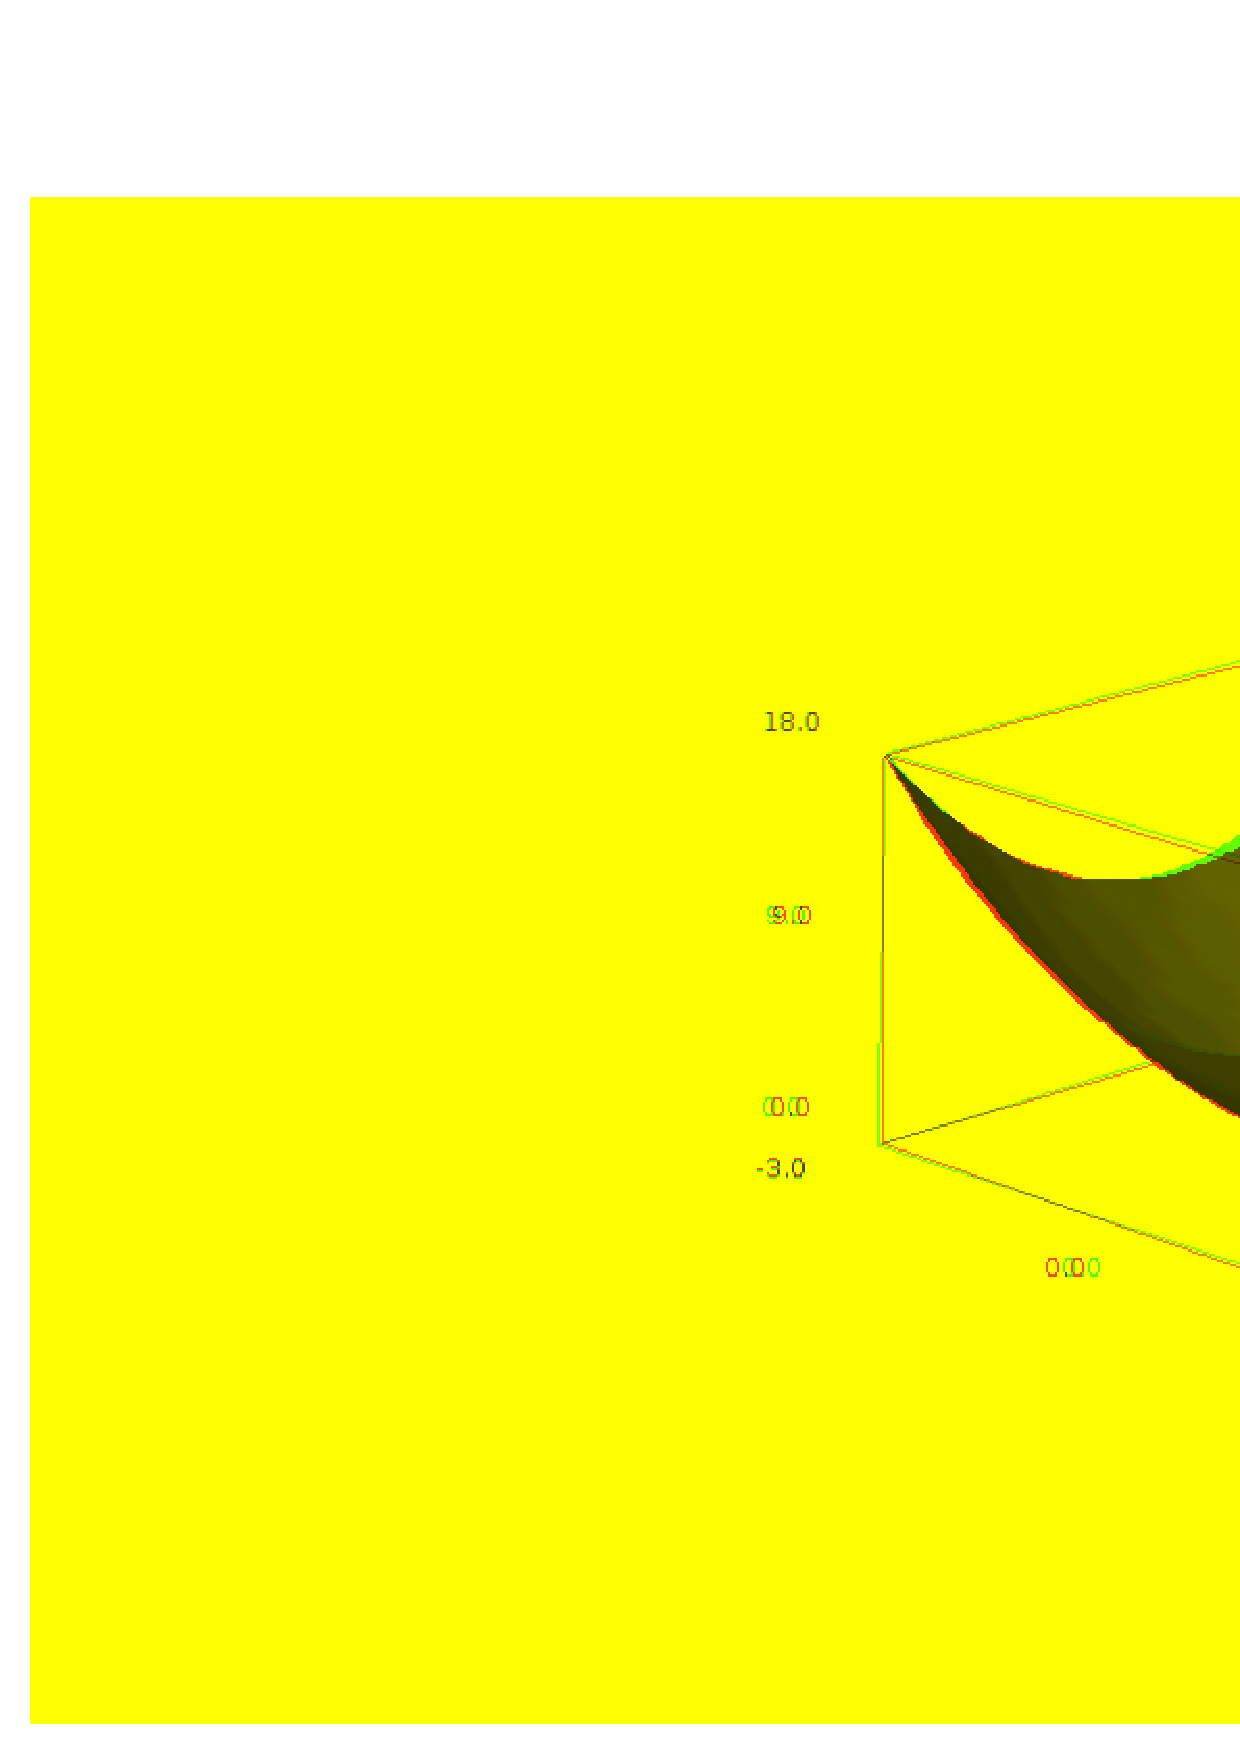
\includegraphics[width=15cm]{pictures_bitmap/coupe.png}
	\end{center}
	À part que l'ordinateur l'a dit, est-ce qu'on peut comprendre pourquoi le graphe de la fonction $x^2+y^2$ ressemble à un bol ? En coordonnées cylindriques, le graphe s'écrit
	\begin{equation}
		z=r^2.
	\end{equation}
	Donc il se fait que plus on s'éloigne du point $(0,0)$ dans le plan $XY$, plus le graphe va monter. Et il monte à quelle vitesse ? Il monte à la vitesse $r^2$. Il s'agit donc de dessiner la fonction $z=r^2$ dans le plan et de la «faire tourner».

\end{example}

%---------------------------------------------------------------------------------------------------------------------------
\subsection{Courbes de niveau}
%---------------------------------------------------------------------------------------------------------------------------

Une technique utile pour se faire une idée de la forme d'une fonction en trois dimensions est de tracer les \defe{courbes de niveau}{courbe de niveau}. La courbe de niveau de hauteur $h$ est la courbe dans le plan donnée par l'équation
\begin{equation}
	f(x,y)=h.
\end{equation}

\begin{example}

	Dessinons par exemple les courbes de niveau de la fonction
	\begin{equation}
		f(x,y)=x+y+2.
	\end{equation}
	La courbe de niveau $h$ est donnée par l'équation $x+y+2=h$, c'est-à-dire
	\begin{equation}
		y(x)=-x+h-2.
	\end{equation}
	Par conséquent la courbe de niveau de hauteur $0$ est $y=-x-2$, celle de hauteur $5$ est $y=-x+3$, etc.

	Nous pouvons également nous aider de Sage pour ce faire :
	\begin{verbatim}
----------------------------------------------------------------------
| Sage Version 4.6.1, Release Date: 2011-01-11                       |
| Type notebook() for the GUI, and license() for information.        |
----------------------------------------------------------------------
sage: f(x,y)=x+y+2
sage: var('h')
h
sage: niveau(h,x)=solve(f(x,y)==h,y)[0].rhs()
sage: g1(x)=niveau(1,x)
sage: g1
x |--> -x - 1
    \end{verbatim}
	Ici la fonction \verb+g1+ est la courbe de niveau $1$.

	Si on veut faire tracer une courbe de niveau, Sage peut le faire :
	\begin{verbatim}
        sage: implicit_plot(f(x,y)==1,(x,-3,3),(y,-4,4))
    \end{verbatim}
	Cela tracera la courbe de niveau $h=1$ dans la partie du plan $x\in\mathopen[ -3 , 3 \mathclose]$ et $y\in\mathopen[ -4,4 ,  \mathclose]$.

\end{example}

Il est bien entendu possible de créer automatiquement $50$ courbes de niveau et de demander de les tracer toutes sur le même graphe.
\lstinputlisting{tex/frido/courbeNiveau.py}

Le résultat est :

\begin{center}
	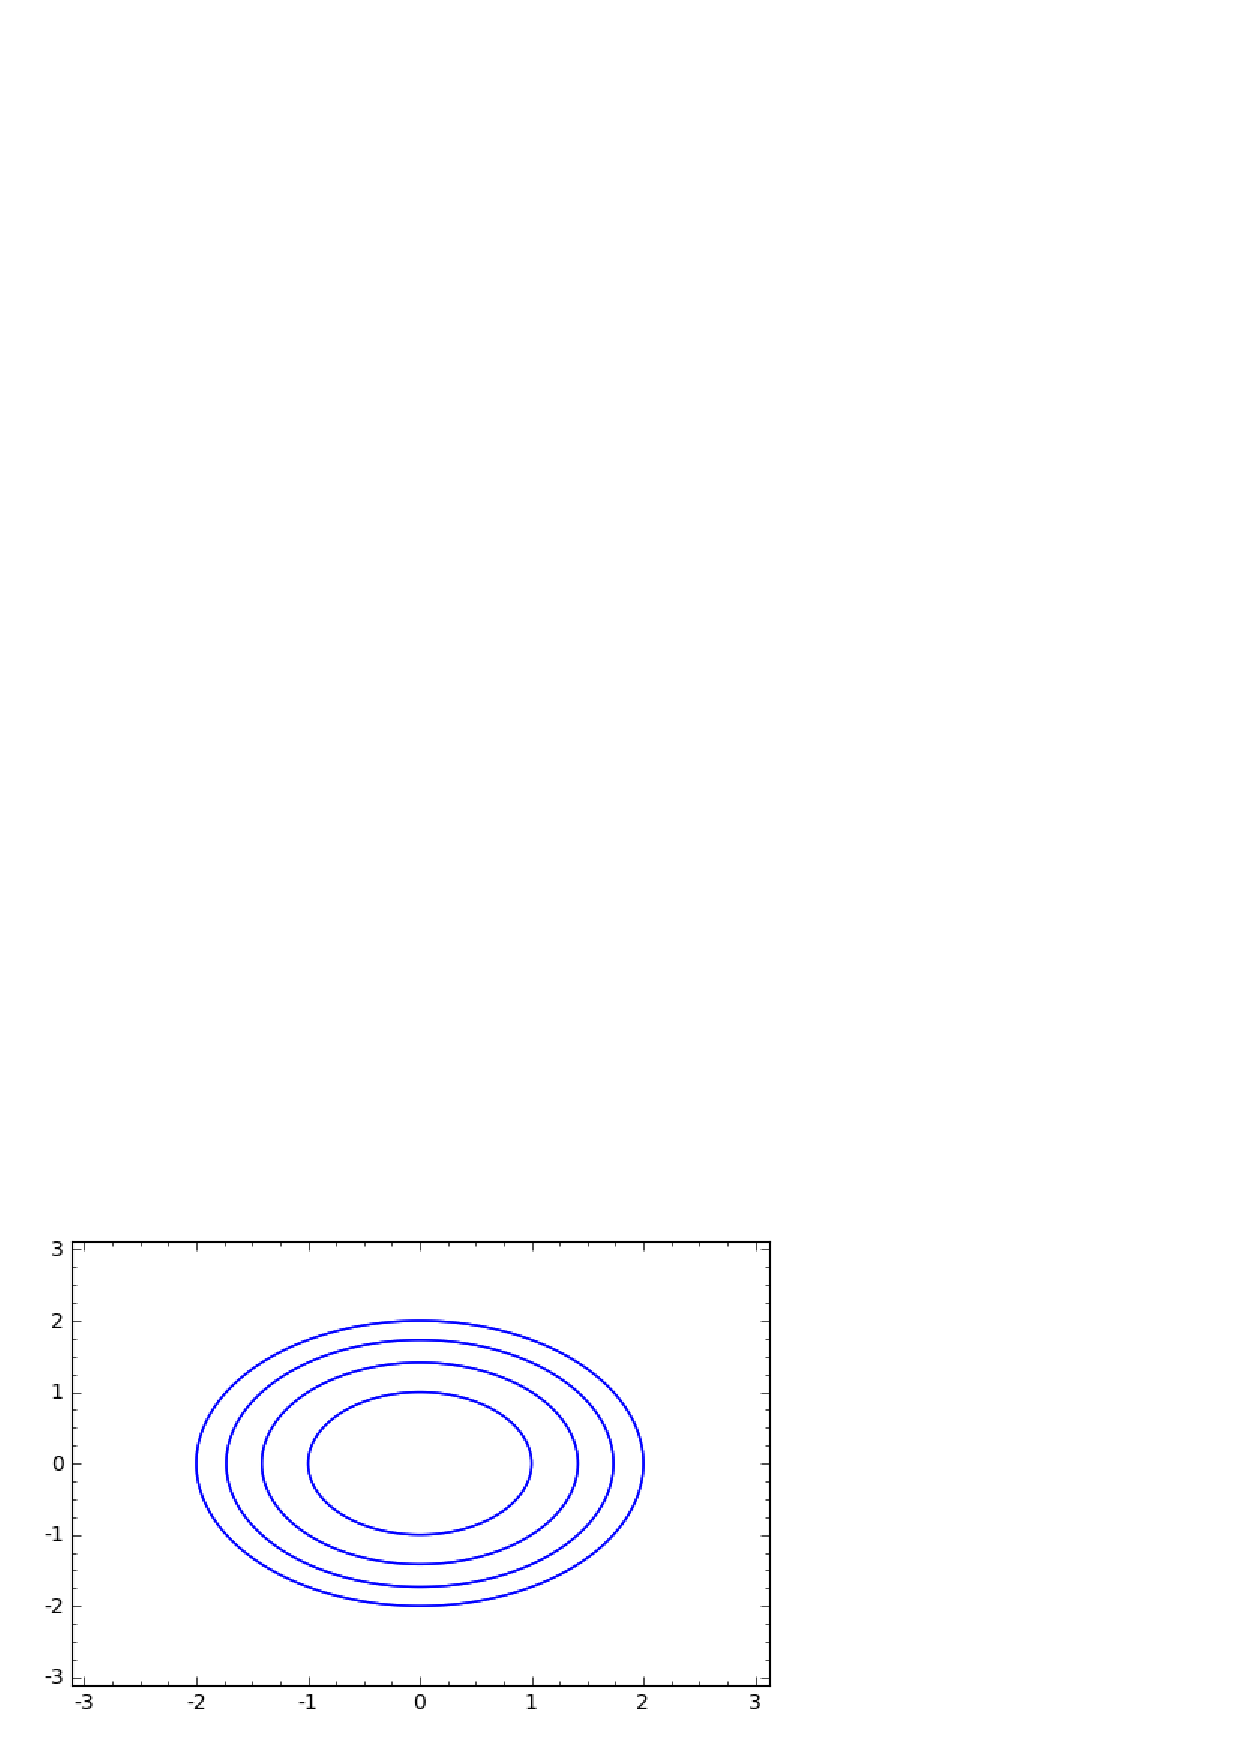
\includegraphics[width=8cm]{pictures_bitmap/niveauCercles.png}
\end{center}
Notez que les courbes sont censées être des cercles : les axes $X$ et $Y$ n'ont pas la même échelle.

\begin{example}
	Un exemple plus riche en enseignements est celui de la fonction
	\begin{equation}
		f(x,y)=x^2-y^2.
	\end{equation}
	La courbe de niveau $h$ est donnée par l'équation $x^2-y^2=h$.

	Commençons par $h=0$. Dans ce cas nous avons $(x+y)(x-y)=0$ et par conséquent les courbes de niveau de hauteur zéro sont les deux droites $x+y=0$ et $x-y=0$.

	Voyons ensuite la courbe de niveau $h=1$. Cela est l'équation $x^2-y^2=1$, c'est-à-dire
	\begin{equation}
		y(x)=\pm\sqrt{x^2-1}.
	\end{equation}
	C'est une fonction qui n'est définie que pour $| x |\geq 1$. Avec $x=1$ nous avons $y=1$. Ensuite, lorsque $x$ grandit, $y$ grandit également, mais la courbe ne peut pas croiser la courbe de niveau $h=0$. Donc, suivant les notations de la figure~\ref{LabelFigCQIXooBEDnfK}, la courbe de niveau «part» de $P$ et doit monter sans croiser les diagonales.

	% les figures CQIXooBEDnfK et KGQXooZFNVnW sont générées par le script MBFDooRFPyNW

	%The result is on figure~\ref{LabelFigCQIXooBEDnfK}. % From file CQIXooBEDnfK
	\newcommand{\CaptionFigCQIXooBEDnfK}{La courbe de niveau $h=1$ de $x^2-y^2$. Notez qu'elle est en deux morceaux.}
	\input{auto/pictures_tex/Fig_CQIXooBEDnfK.pstricks}

	%The result is on figure~\ref{LabelFigKGQXooZFNVnW}. % From file KGQXooZFNVnW
	\newcommand{\CaptionFigKGQXooZFNVnW}{La courbe de niveau $x^2-y^2=-1$.}
	\input{auto/pictures_tex/Fig_KGQXooZFNVnW.pstricks}

	En ce qui concerne la courbe de niveau $h=-1$, elle correspond à la courbe $y=\pm\sqrt{1+x^2}$ qui est définie pour tous les $x\in\eR$. Le même raisonnement que précédemment nous amène à la figure~\ref{LabelFigKGQXooZFNVnW}.

\end{example}

Une autre façon de voir les courbes de niveau est de dire que la courbe de niveau de hauteur $h$ est la projection dans le plan $XY$ de la section du graphe de $f$ par le plan $z=h$.

On peut également définir le graphe de fonctions de trois (ou plus) variables. Le graphe de la fonction $f\colon D\subset\eR^3\to \eR$ est l'ensemble
\begin{equation}
	\big\{ \big( x,y,z,f(x,y,z) \big)\tq (x,y,z)\in D \big\}\subset \eR^4.
\end{equation}
De tels graphes ne peuvent pas être représentés sur une feuille de papier. Il est toutefois possible de définir les ensembles de niveaux :
\begin{equation}
	E_h=\big\{ (x,y,z)\in D\tq  f(x,y,z)=h\big\}.
\end{equation}
Ce sont des surfaces dans $\eR^3$ que l'on peut dessiner.

\begin{example}
	Les surfaces de niveau de la fonction $f(x,y,z)=x^2+y^2+z^2$ sont des sphères. Il n'y a pas de surfaces de niveau pour les «hauteurs» négatives.
\end{example}

\begin{example}
	Considérons la fonction $f(x,y,z)=x^2+y^2-z^2$. En coordonnées cylindriques, cette fonction s'écrit
	\begin{equation}
		f(r,\theta,z)=r^2-z^2.
	\end{equation}
	La surface de niveau $0$ est donnée par l'équation $r=| z |$. Cela fait un cercle à chaque hauteur, dont le rayon grandit linéairement avec la hauteur; le tout est donc un cône. C'est d'ailleurs le cône obtenu par rotation de la courbe de niveau $h=0$ que nous avions obtenu pour la fonction $x^2-y^2$.

	En ce qui concerne les ensembles de niveau positifs, ils sont donnés par
	\begin{equation}
		z=\pm\sqrt{x^2+y^2-h}.
	\end{equation}
	Notez qu'ils ne sont pas définis pour $r\geq h$. Cela pose un petit problème quand on veut le tracer à l'ordinateur :
	\begin{verbatim}
----------------------------------------------------------------------
| Sage Version 4.6.1, Release Date: 2011-01-11                       |
| Type notebook() for the GUI, and license() for information.        |
----------------------------------------------------------------------
sage: var('x,y')
(x, y)
sage: f(x,y)=sqrt(x**2+y**2-3)
sage: F=plot3d(f(x,y),(x,-5,5),(y,-5,5))
sage: G=plot3d(-f(x,y),(x,-5,5),(y,-5,5))
sage: F+G
    \end{verbatim}
	Le résultat est\footnote{Encore une fois : ça donne mieux à l'écran, et vous pouvez le faire bouger; je vous encourage à le faire !} :
	\begin{center}
		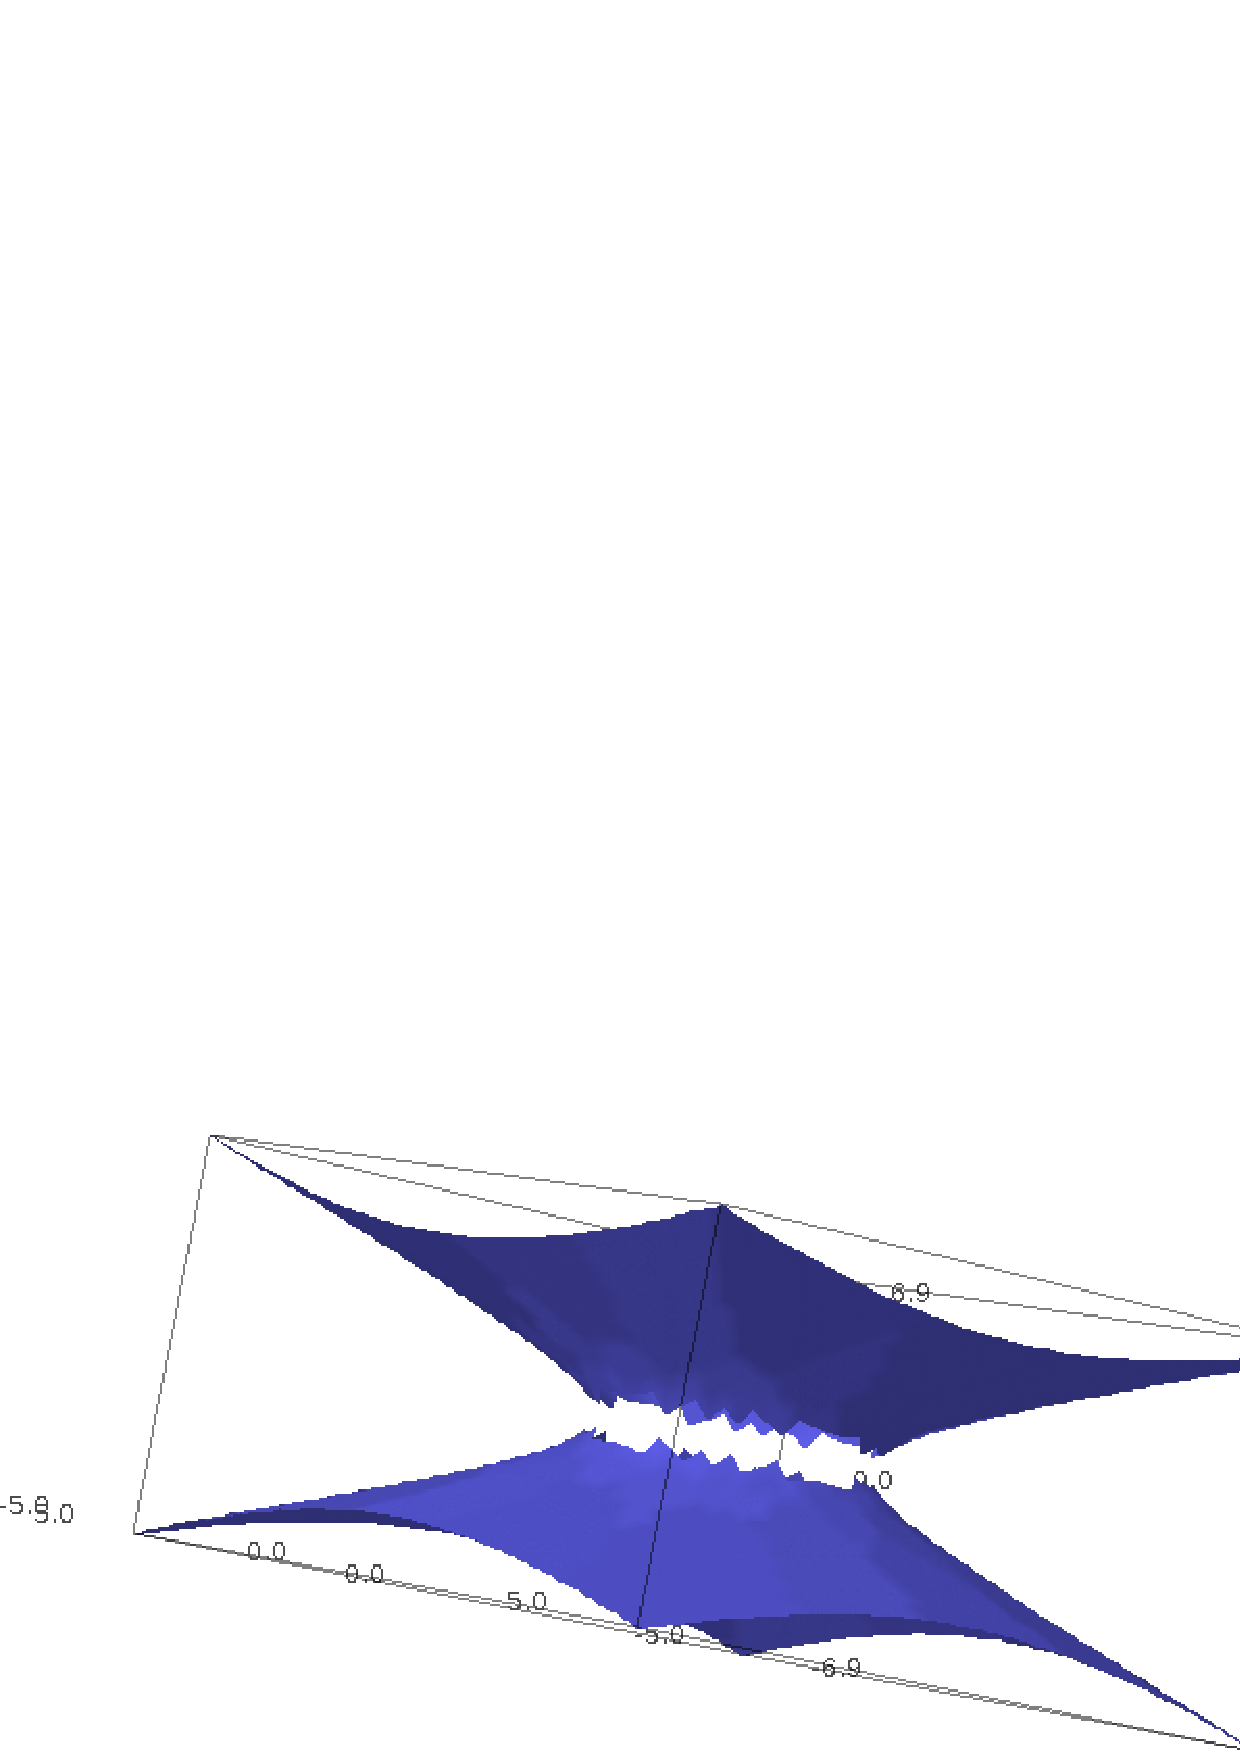
\includegraphics[width=15cm]{pictures_bitmap/AdSmauvais.png}
	\end{center}
	On voit qu'il y a un grand trou au centre correspondant aux $z$ proches de zéro. Or d'après l'équation, il n'en est rien : en $z=0$ il y a bel et bien tout un cercle. Afin d'obtenir une meilleur image, il faut demander de tracer avec un maillage plus fin :
	\begin{verbatim}
----------------------------------------------------------------------
| Sage Version 4.6.1, Release Date: 2011-01-11                       |
| Type notebook() for the GUI, and license() for information.        |
----------------------------------------------------------------------
sage: var('x,y')
(x, y)
sage: f(x,y)=sqrt(x**2+y**2-3)
sage: F=plot3d(f(x,y),(x,-5,5),(y,-5,5),plot_points=300)
sage: G=plot3d(-f(x,y),(x,-5,5),(y,-5,5),plot_points=300)
sage: F+G
    \end{verbatim}
	Le temps de calcul est un peu plus long, mais le résultat est meilleur :
	\begin{center}
		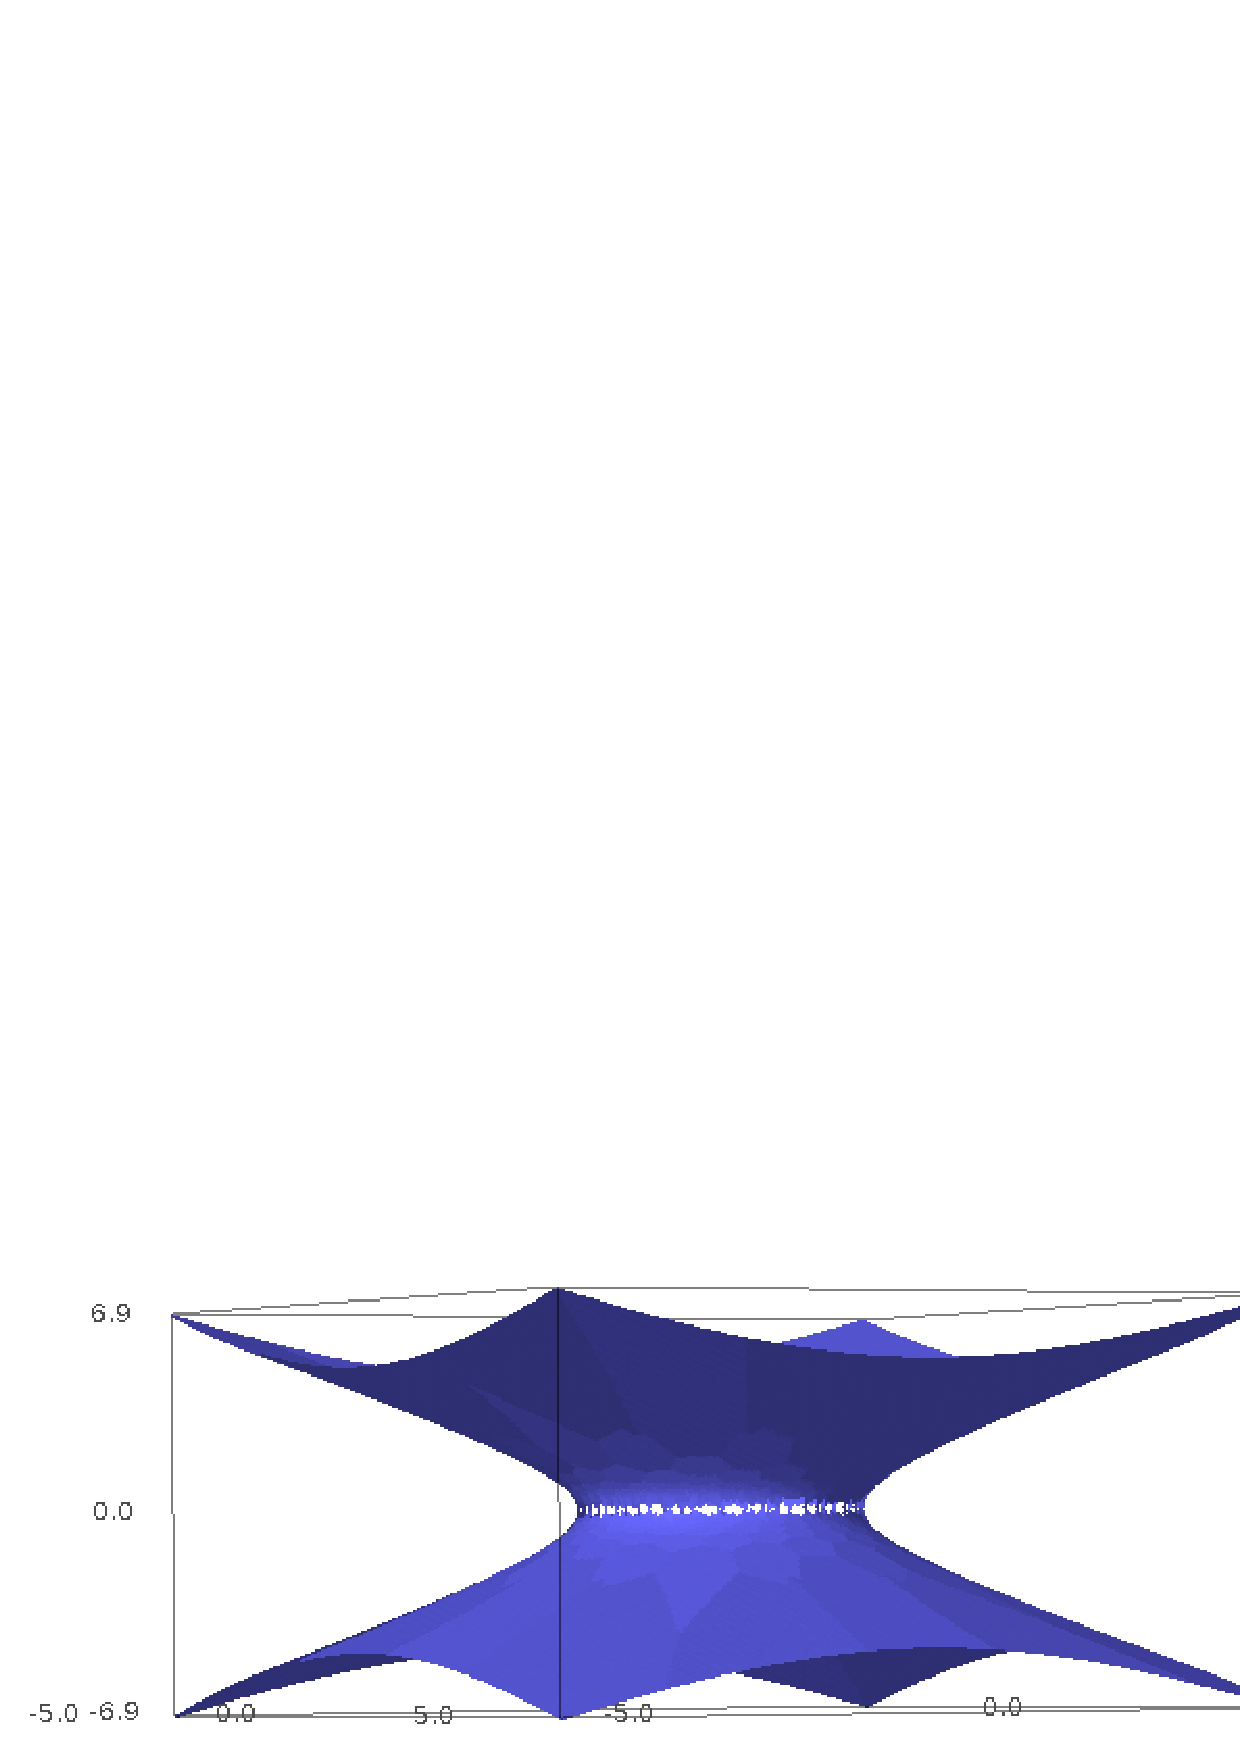
\includegraphics[width=15cm]{pictures_bitmap/AdSbon.png}
	\end{center}
\end{example}

%+++++++++++++++++++++++++++++++++++++++++++++++++++++++++++++++++++++++++++++++++++++++++++++++++++++++++++++++++++++++++++
%\section{Calcul de limites}
%+++++++++++++++++++++++++++++++++++++++++++++++++++++++++++++++++++++++++++++++++++++++++++++++++++++++++++++++++++++++++++

%Incidemment, le lemme~\ref{Def_diff2} nous donne une nouvelle technique pour calculer des limites à plusieurs variables, similaire à celle du développement asymptotique expliquée dans la section~\ref{SecTaylorR}.

%En effet, la formule \eqref{def_diff2} nous permet d'écrire $f(x)$ sous la forme
%\begin{equation}
%	f(x)=f(a)+df(a).(x-a)+\sigma_f(a,x)\| x-a \|
%\end{equation}
%où la fonction $\sigma_f$ satisfait $\lim_{x\to a}\sigma_f(a,x)=0$. Ici, $x$ et $a$ sont des éléments de $\eR^m$.

%+++++++++++++++++++++++++++++++++++++++++++++++++++++++++++++++++++++++++++++++++++++++++++++++++++++++++++++++++++++++++++
\section{Limites à plusieurs variables}
%+++++++++++++++++++++++++++++++++++++++++++++++++++++++++++++++++++++++++++++++++++++++++++++++++++++++++++++++++++++++++++
\label{SecLimVarsPlus}

Prenons une fonction $f\colon \eR^n\to \eR$. Nous disons que
\begin{equation}
	\lim_{x\to x_0}f(x)=l\in\eR
\end{equation}
lorsque $\forall \epsilon>0$, $\exists\delta$ tel que $\| x-x_0 \|\leq\delta$ implique $| f(x)-l |\leq \epsilon$.

Remarquez qu'ici, $x\in\eR^n$, et sachez distinguer $\| . \|$, la norme dans $\eR^n$ de $| . |$ qui est la valeur absolue dans $\eR$. Une autre façon d'exprimer cette définition est que l'ensemble des valeurs atteintes par $f$ dans une boule de rayon $\delta$ autour de $x_0$ n'est pas très loin de $l$. Nous définissons donc
\begin{equation}
	E_{\delta}=\{ f(x)\tq x\in B(x_0,\delta) \}.
\end{equation}
Notez que si $f$ n'est pas définie en $x_0$, il n'y a pas de valeurs correspondantes au centre de la boule dans $E_{\delta}$. Ceci est évidemment la situation générique lorsqu'il y a une indétermination à lever dans le calcul de la limite. Nous avons alors que
\begin{equation}
	\lim_{x\to x_0}f(x)=l
\end{equation}
lorsque $\forall\epsilon>0$, $\exists\delta$ tel que
\begin{equation}        \label{Eqvmoinsrapplimdeux}
	\sup\{ | v-l |\tq v\in E_{\delta} \}\leq\epsilon.
\end{equation}
Une façon classique de montrer qu'une limite n'existe pas, est de prouver que, pour tout $\delta$, l'ensemble $E_{\delta}$ contient deux valeurs constantes. Si par exemple $0\in E_{\delta}$ et $1\in E_{\delta}$ pour tout $\delta$, alors aucune valeur de $l$ (même pas $l=\pm\infty$) ne peut satisfaire à la condition \eqref{Eqvmoinsrapplimdeux} pour toute valeur de $\epsilon$.

Nous laissons à la sagacité de l'étudiant le soin d'adapter tout ceci pour le cas $\lim_{x\to x_0}f(x)=\pm\infty$.

La proposition suivante semble évidente, mais nous sera tellement
utile qu'il est préférable de l'expliciter~:
\begin{proposition}     \label{PROPooPOAQooPmxEtb}
	Soient $f : D \to \eR$ une fonction de domaine \( D\), \( a\in\Adh(D)\) et un voisinage \( V\) de \( a\). Nous supposons que \( V\cap D\) s'écrive comme une intersection finie :
	\begin{equation*}
		V\cap D = \bigcup_{i=1}^k A_i
	\end{equation*}
	telle que $a \in \Adh A_i$ pour tout $i \leq k$. Alors, la limite
	\begin{equation}      \label{EQooEXELooHccCGw}
		\limite x a f(x)
	\end{equation}
	existe et vaut $b\in \eR$ si et seulement si chacune des limites
	\begin{equation}
		\limite[x \in A_i] x a f(x)
	\end{equation}
	existe et vaut $b$.
\end{proposition}

\begin{proof}On sait déjà que si la limite de $f : D \to \eR$
	existe, alors toute restriction à $A_i$ admet la même limite\footnote{C'est une conséquence de la caractérisation séquentielle de la continuité \ref{fContEstSeqCont}.}. Il suffit donc de prouver la réciproque.

	Fixons provisoirement un entier \( i\) entre \( 1\) et \( k\) ainsi que \( \epsilon>0\). Vu que \( \lim_{\substack{x\to a\\x\in A_i}} f(x)=b\), il existe \( \delta_i>0\) tel que si \( x\in A_i\) et si \( 0<| x-a |<\delta_i\), alors
	\begin{equation}        \label{EQooUCAIooRpUgnE}
		| f(x)-f(a) |<\epsilon.
	\end{equation}
	Quitte à prendre \( \delta_i\) un peu plus petit, nous supposons que \( V\subset B(a,\delta_i)\).

	Nous posons $\delta = \min\{\delta_i\}_{i=1,\ldots, k}$, et nous considérons \( x\in D\) tel que \( 0<| x-a |<\delta\). Nous avons alors
	\begin{enumerate}
		\item \( x\in V\cap D\),
		\item il existe \( i\) tel que \( x\in A_i\).
	\end{enumerate}
	Ce \( x\) est donc un élément de \( A_i\) vérifiant \( 0<| x-a |<\delta\leq \delta_i\). Il vérifie donc \eqref{EQooUCAIooRpUgnE} : \( | f(x)-f(a) |<\epsilon\).

	Cela prouve la limite \eqref{EQooEXELooHccCGw}.
\end{proof}

\begin{example}
	\begin{enumerate}
		\item Pour qu'une fonction $f : \eR \to \eR$ admette une limite en $a \in \eR$, il faut et il suffit qu'elle y admette une limite à droite et une limite à gauche qui soient égales.

		      Cela est une application de la proposition \ref{PROPooPOAQooPmxEtb} avec \( \eR=\mathopen] -\infty , a \mathclose[\cup\mathopen] a , \infty \mathclose[\).

		\item Une suite $(x_k)$ admet une limite si et seulement si les
		      sous-suites $(x_{2k})$ et $(x_{2k+1})$ convergent vers la même
		      limite. Ceci n'est pas une application directe de la proposition,
		      mais la teneur est la même.
	\end{enumerate}
\end{example}

\begin{lemma}[\cite{MonCerveau}]
	Soient deux espaces vectoriels \( E\) et \( F\). Soit une fonction \( f\colon \eR\to F\) telle que \( \lim_{t\to 0} f(t)=y\in F\). Nous posons
	\begin{equation}
		\begin{aligned}
			\varphi\colon E & \to F               \\
			h               & \mapsto f(\| h \|).
		\end{aligned}
	\end{equation}
	Alors \( \varphi\) admet une limite pour \( h\to 0\) et elle est donnée par
	\begin{equation}
		\lim_{h\to 0} \varphi(h)=\lim_{t\to 0} f(t).
	\end{equation}
\end{lemma}

\begin{proof}
	Soit \( \epsilon>0\). Il existe \( \delta\) tel que si \( t<\delta\) alors \( \| f(t)-y \|_F<\epsilon\). Si \( \| h \|<\delta\) nous avons
	\begin{equation}
		\| \varphi(h)-y \|=\| f(\| h \|)-y \|<\epsilon.
	\end{equation}
	Donc c'est bon.
\end{proof}

Voici, dans le même ordre d'idée, un autre résultat qui permet de réduire le nombre de variables dans une limite lorsque la fonction ne dépend pas de certaines variables.

\begin{lemma}[\cite{MonCerveau}]        \label{LEMooYLIHooFBQyzC}
	Soit une fonction \( g\colon \eR\to \eR\) vérifiant
	\begin{equation}
		\lim_{t\to a} g(t)=\ell.
	\end{equation}
	Alors la fonction
	\begin{equation}
		\begin{aligned}
			f\colon \eR^2 & \to \eR      \\
			(x,y)         & \mapsto g(x)
		\end{aligned}
	\end{equation}
	vérifie
	\begin{equation}
		\lim_{\substack{(x,y)\to(a,b)\\x\neq a}} f(x,y)=\ell.
	\end{equation}
\end{lemma}

\begin{proof}
	Soit \( \epsilon>0\). Par hypothèse sur la limite de \( g\) en \( a\), il existe \( \delta>0\) tel que \( 0<| t-a |<\delta\) implique \( | g(t)-\ell |<\epsilon\).

	Attention : passage subtil\footnote{Je rejette déjà en bloc et d'un revers de main toute tentative de dire «la limite épointée, c'est mieux». Voir aussi l'exemple \ref{EXooHSYNooBZhDbE}.}.  Si \( 0<\| (x,y)-(a,b) \|<\delta\), alors nous avons évidemment aussi \( | x-a |<\delta\), mais pas spécialement \( 0<| x-a |<\delta\) comme le requis pour utiliser la limite de \( g\).

	Dans le calcul de la limite restreinte à \( x\neq a\), les points qui interviennent sont les valeurs de \( (x,y)\) dans \( B\big( (a,b),\delta \big)\setminus\{ x=a \}\). Or pour celles-là nous avons bien \( 0<| x-a |<\delta\). Le calcul suivant fonctionne donc :
	\begin{equation}
		| f(x,y)-\ell |=| g(x)-\ell |<\epsilon.
	\end{equation}
\end{proof}

\begin{example}     \label{EXooHSYNooBZhDbE}
	Pourquoi prendre la limite \( (x,y)\to (a,b)\) avec \( x\neq a\) dans l'énoncé du lemme \ref{LEMooYLIHooFBQyzC} ? Imaginons la fonction
	\begin{equation}
		g(x)=\begin{cases}
			0 & \text{si } x\neq 0 \\
			1 & \text{si } x=0.
		\end{cases}
	\end{equation}
	Dans ce cas, le graphe de la fonction \( f(x,y)=g(x)\) est tout plat sauf la ligne \( x=0\) qui est en hauteur. Nous avons donc \( f(0,t)=1\) pour tout \( t\) et donc nous n'avons pas \( \lim_{(x,y)\to (0,0)} f(x,y)=0\) :  tout voisinage de \( (0,0)\) contient des points \( (x,y)\) tels que \( f(x,y)=1\) et des points \( (x,y)\) tels que \( f(x,y)=0\).
\end{example}

Il existe de nombreuses façons de calculer des limites à plusieurs variables. Plus nous connaîtrons de mathématiques, plus nous aurons de techniques à notre disposition. Nous allons tout de suite voir quelques méthodes. Voir le thème~\ref{THEMEooLTCIooGDIPnF} pour plus de techniques et d'exemples.

%--------------------------------------------------------------------------------------------------------------------------- 
\subsection{Caractérisation de la limite par les suites}
%---------------------------------------------------------------------------------------------------------------------------

\begin{example}		\label{ExFNExempleMethodeTrigigi}
	Considérons la fonction
	\begin{equation}
		f(x,y)=\frac{ xy }{ x^2+y^2 },
	\end{equation}
	et remarquons que, quelle que soit la valeur de $y$, cette fonction est nulle lorsque $x=0$. De la même manière, nous voyons que si $x=y$, alors la fonction vaut\footnote{En fait ce que nous sommes en train de faire est de poser $\theta=\pi/2$ et $\theta=\pi/4$ dans \eqref{Eq2807fpolairerhodeuxcossin}.} $\frac{ 1 }{2}$.

	Il est impossible que la fonction ait une limite en $(0,0)$ parce qu'on ne peut pas trouver un $\ell$ dont on s'approche à la fois en suivant la ligne $x=0$ et la ligne $x=y$.

	Deux autres chemins avec encore deux autres valeurs sont dessinés sur la figure~\ref{LabelFigMethodeChemin}.

	Cet exemple pourra être formalisé en utilisant le théorème~\ref{ThoLimSuite}. Voir l'exemple~\ref{EXooNBTYooFyKRTB}.
\end{example}

\begin{theorem}[Caractérisation de la limite par les suites]		\label{ThoLimSuite}
	Une fonction $f\colon D\subset\eR^m\to \eR^n$ admet une limite $\ell$ en un point d'accumulation $a$ de $D$ si et seulement si pour toute suite $(x_n)$ dans $D\setminus\{ a \}$ convergente vers $a$, la suite $\big( f(x_n) \big)$ dans $\eR^n$ converge vers $\ell$.
\end{theorem}

\begin{proof}
	Supposons d'abord que la fonction ait une limite $\ell$ lorsque $x\to a$, et considérons une suite $(x_n)$ dans $D\setminus\{ a \}$ convergente vers $a$. Nous devons montrer que la suite $y_n=f(x_n)$ converge vers $\ell$, c'est-à-dire que si nous choisissons $\varepsilon>0$ nous devons montrer qu'il existe un $N$ tel que $n>N$ implique $\| y_n-\ell  \|=\| f(x_n)-\ell \|<\varepsilon$.

	Nous avons deux hypothèses. La première est la convergence de la fonction et la seconde est la convergence de la suite $(x_n)$. L'hypothèse de convergence de la fonction nous dit que (le $\varepsilon$ a déjà été choisi dans le paragraphe précédent)
	\begin{equation}
		\exists\delta\tq\,0<\| x-a \|<\delta\Rightarrow\| f(x)-\ell \|<\varepsilon.
	\end{equation}
	Une fois choisi ce $\delta$ qui «va avec» le $\varepsilon$ qui a été choisi précédemment, la définition de la convergence de la suite nous enseigne que
	\begin{equation}
		\exists N\tq n>N\Rightarrow\| x_n-a \|<\delta.
	\end{equation}
	Récapitulons ce que nous avons fait. Nous avons choisi un $\varepsilon$, et puis nous avons construit un $N$. Lorsque $n>N$, nous avons $\| x_n-a \|<\delta$. Mais alors, par construction de ce $\delta$, nous avons $\| f(x_n)-\ell \|<\varepsilon$. Au final, $n>N$ implique bien $\| y_n-\ell \|<\varepsilon$, ce qu'il nous fallait.

	Nous supposons maintenant que la fonction $f$ \emph{ne} converge \emph{pas} vers $\ell$, et nous allons construire une suite d'éléments $x_n$ qui converge vers $a$ sans que $(y_n)=f(x_n)$ ne converge vers $\ell$. La fonction $f$ vérifie la condition \eqref{EqCaractNonLim}. Nous prenons donc un $\varepsilon$ tel que $\forall \delta$, il existe un $x$ qui vérifie \emph{en même temps} les deux conditions
	\begin{subequations}
		\begin{numcases}{}
			0<\| x-a \|<\delta\\
			\| f(x)-\ell \|>\varepsilon.
		\end{numcases}
	\end{subequations}
	Un tel $x$ existe pour tout choix de $\delta$. Choisissons un $n$ arbitraire et $\delta=\frac{1}{ n }$. Nous nommons $x_n$ le $x$ correspondant à ce choix de $n$. La suite $(x_n)$ ainsi construite converge vers $a$ parce que
	\begin{equation}
		\| x_n-a \|<\delta_n=\frac{1}{ n },
	\end{equation}
	donc dès que $n$ est grand, $\| x_n-a \|$ est petit. Mais la suite $y_n=f(x_n)$ ne converge pas vers $\ell$ parce que
	\begin{equation}
		\| f(x_n)-\ell \|>\varepsilon
	\end{equation}
	pour tout $n$. La suite $y_n$ ne s'approche donc jamais à moins d'une distance $\varepsilon$ de $\ell$.
\end{proof}

\begin{example} \label{EXooNBTYooFyKRTB}
	Reprenons l'exemple \ref{ExFNExempleMethodeTrigigi}. Considérons les deux suites $x_n=(0,\frac{1}{ n })$ et $y_n=(\frac{1}{ n },\frac{1}{ n })$. Ce sont deux suites dans $\eR^2$ qui tendent vers $(0,0)$. Si la fonction $f$ convergeait vers $\ell$, alors nous aurions au moins
	\begin{subequations}\label{Eq3007Lixxyyell}
		\begin{align}
			\lim f(x_n) & =\ell  \\
			\lim f(y_n) & =\ell,
		\end{align}
	\end{subequations}
	mais nous savons que pour tout $n$, $f(x_n)=f(0,\frac{1}{ n })=0$ et $f(y_n)=f(\frac{1}{ n },\frac{1}{ n })=\frac{1}{ 2 }$. Il n'y a donc aucun nombre $\ell$ qui vérifie les deux équations \eqref{Eq3007Lixxyyell} parce que $\lim f(x_n)=0$ et $\lim f(y_n)=\frac{ 1 }{2}$.
\end{example}

%---------------------------------------------------------------------------------------------------------------------------
\subsection{Règle de l'étau}
%---------------------------------------------------------------------------------------------------------------------------

Une première façon de calculer la limite d'une fonction est de la «coincer» entre deux fonctions dont nous connaissons la limite.
\begin{theorem}[Règle de l'étau\cite{BIBooNKECooNNYQvB}]		\label{ThoRegleEtau}
	Soit $\mO$, un ouvert de $\eR^m$ contenant le point $a$. Soient $f$, $g$ et $h$, trois fonctions définies sur $\mO$ (éventuellement pas en $a$ lui-même). Supposons que pour tout $x\in\mO$ (à part éventuellement $a$), nous ayons les inégalités
	\begin{equation}
		g(x)\leq f(x)\leq h(x).
	\end{equation}
	Supposons de plus que
	\begin{equation}
		\lim_{x\to a} g(x)=\lim_{x\to a} h(x)=\ell.
	\end{equation}
	Alors la limite $\lim_{x\to a} f(x)$ existe et vaut $\ell$.
\end{theorem}

Nous insistons sur le fait que les deux fonctions entre lesquelles nous coinçons $f$ doivent tendre vers \emph{la même} valeur.

Cette méthode est très pratique lorsqu'on a des fonctions trigonométriques qui se factorisent parce qu'elles sont toujours majorables par $1$; voir l'exemple~\ref{EXooSPFDooSluUGV}.

\begin{example}
	Prouver la continuité en $(0,0)$ de la fonction
	\begin{equation}
		f(x,y)=\begin{cases}
			\frac{ x | y | }{ \sqrt{x^2+y^2} } & \text{si }(x,y)\neq (0,0) \\
			0                                  & \text{sinon.}
		\end{cases}
	\end{equation}
	Considérons une suite $(x_n,y_n)\in\eR^2$ qui tend vers $(0,0)$. Étant donné que $\frac{ | y | }{ \sqrt{x^2+y^2} }<1$ pour tout $x$ et $y$, nous avons
	\begin{equation}
		0\leq | f(x_n,y_n) |=\left| \frac{ x_n | y_n | }{ \sqrt{x_n^2+y_n^2} } \right| \leq | x_n |\to 0.
	\end{equation}
	Donc nous avons
	\begin{equation}
		\lim_{(x,y)\to(0,0)}f(x,y)=0=f(0,0),
	\end{equation}
	ce qui prouve que la fonction est continue en $(0,0)$ par la proposition~\ref{PropFnContParSuite}. Nous avons utilisé la règle de l'étau (théorème~\ref{ThoRegleEtau}).
\end{example}

\begin{normaltext}
	Nous notons \( f\sim g\)\nomenclature[Y]{\( f\sim g\)}{fonctions ayant des limites équivalentes} pour \( x\to a\) lorsque \( \lim_{x\to a} \frac{ f(x) }{ g(x) }=1\).

	Cela signifie que \( f\) et \( g\) tendent vers la même limite, à la même vitesse.
\end{normaltext}

%---------------------------------------------------------------------------------------------------------------------------
\subsection{Méthode des chemins}
%---------------------------------------------------------------------------------------------------------------------------

Lorsque la limite n'existe pas, il y a une façon en général assez simple de le savoir, c'est la \defe{méthode des chemins}{méthode!des chemins}.

\newcommand{\CaptionFigMethodeChemin}{Sur toute la droite $y=-x$, la fonction vaut $-1/2$, tandis que sur toute la droite $y=x/2$, elle vaut $\frac{2}{ 5 }$. Il est donc impossible que la fonction ait une limite en $(0,0)$, parce que dans toute boule autour de zéro, il y aura toujours un point de chacune de ces deux droites.}
\input{auto/pictures_tex/Fig_MethodeChemin.pstricks}

C'est la proposition suivante qui va faire une grosse partie du travail.
\begin{proposition}[\cite{MonCerveau}]     \label{PROPooSAFIooWvmSiT}
	Soit $f\colon D\subset\eR^m\to \eR^n$ et $a$ un point d'adhérence de $D$. Alors nous avons
	\begin{equation}
		\lim_{x\to a} f(x)=\ell
	\end{equation}
	si et seulement si pour toute fonction $\gamma\colon \eR\to \eR^m$ telle que $\lim_{t\to 0} \gamma(t)=a$, nous avons
	\begin{equation}
		\lim_{t\to 0} (f\circ\gamma)(t)=\ell.
	\end{equation}
\end{proposition}

\begin{proof}
	En deux parties.
	\begin{subproof}
		\item[Sens direct]
		Soit une fonction \( \gamma\colon \eR\to \eR^m\) telles que \( \lim_{t\to 0} \gamma(t)=a\). Par le théorème \ref{ThoLimSuite}, il suffit de montrer que \( (f\circ\gamma)(t_n)\to\ell\) pour toute suite \( t_n\to 0\) dans \( \eR\).

		Nous savons que la suite \( n\mapsto \gamma(t_n)\) est une suite qui converge vers \( a\). Mais l'hypothèse \( \lim_{x\to a} f(x)=\ell\) implique que pour toute suite \( x_n\to a\) nous avons \( f(x_n)\to \ell\). Cela est en particulier vrai pour la suite \( n\mapsto \gamma(t_n)\). Donc :
		\begin{equation}
			\lim_{n\to \infty} f\big( \gamma(t_n) \big)=\ell,
		\end{equation}
		ce qu'il fallait prouver.
		\item[Réciproque]

		Pour les mêmes raisons de caractérisation séquentielle que précédemment, il faut prouver que \( \lim_{n\to \infty} f(x_n)=\ell\) pour tout suite \( x_n\to a\).

		\begin{subproof}
			\item[Un chemin]

			Soit la fonction \( \gamma\colon \eR\to \eR^m\) affine par morceaux et telle que
			\begin{equation}
				\gamma\left( \frac{1}{ n } \right)=x_n.
			\end{equation}
			Nous prolongeons \( \gamma\) par \( \gamma(t)=a\) pour \( t\leq 0\).

			\item[\( \gamma(t)\to a\)]

			Nous montrons que \( \lim_{t\to 0} \gamma(t)=a\). Soient \( \epsilon>0\) et \( N\) tel que \( x_n\in B(a,\epsilon)\) pour tout \( n\geq N\). Si \( t<\frac{1}{ N }\) alors \( t\in\mathopen[ \frac{1}{ k+1 } , \frac{1}{ k } \mathclose]\) pour un certain \( k>N\). Donc
			\begin{equation}
				\gamma(t)\in\mathopen[ \gamma(\frac{1}{ k+1 }) , \gamma(\frac{1}{ k }) \mathclose]
			\end{equation}
			et donc \( \gamma(t)\in\mathopen[ x_{k+1} , x_k \mathclose]\) parce que \( \gamma\) est formé de ces segments de droites. Mais comme \( B(a,\epsilon)\) est convexe\footnote{C'est la proposition \ref{PROPooUQLUooDQfYLT}.}, nous avons
			\begin{equation}
				\gamma(t)\in\mathopen[ x_{k+1} , x_k \mathclose]\subset B(a,\epsilon).
			\end{equation}
			Nous avons donc bien \( \lim_{t\to 0} \gamma(t)=a\).
			\item[Conclusion]

			L'hypothèse nous donne alors \( \lim_{t\to 0} (f\circ \gamma)(t)=\ell\). En particulier le critère de la caractérisation séquentielle de la limite dit que
			\begin{equation}
				\lim_{n\to \infty} f\big( \gamma(\frac{1}{ n }) \big)=\ell,
			\end{equation}
			ce qui signifie \( \lim_{n\to \infty} f(x_n)=\ell\).
		\end{subproof}
	\end{subproof}
\end{proof}

\begin{corollary}	\label{CorMethodeChemin}
	Soient $f\colon D\subset\eR^m\to \eR^n$ et $a$ un point d'accumulation de $D$. Si nous avons deux fonctions $\gamma_1,\gamma_2\colon \eR\to \eR^m$ telles que
	\begin{equation}
		\lim_{t\to 0} \gamma_1(t)=\lim_{t\to 0} \gamma_2(t)=a
	\end{equation}
	tandis que
	\begin{equation}
		\lim_{t\to 0} (f\circ \gamma_1)(t)\neq\lim_{t\to 0} (f\circ \gamma_2)(t),
	\end{equation}
	ou bien que l'une des deux limites n'existe pas, alors la limite de $f(x)$ lorsque $x\to a$ n'existe pas.
\end{corollary}

\begin{corollary}	\label{CorMethodeChemoinNegatif}
	Soient $f\colon D\subset\eR^m\to \eR^n$ et $a$ un point d'accumulation de $D$. Si il existe une fonction $\gamma\colon \eR\to \eR^m$ avec $\gamma(0)=a$ telle que la limite $\lim_{t\to 0} (f\circ\gamma)(t)$ n'existe pas, alors la limite $\lim_{x\to a} f(x)$ n'existe pas.
\end{corollary}

En ce qui concerne le calcul de limites, la méthode des chemins peut être utilisé de trois façons :
\begin{enumerate}
	\item
	      Dès que l'on trouve une fonction $\gamma\colon \eR\to \eR^m$ telle que $\lim_{t\to 0} (f\circ \gamma)(t)=\ell$, alors nous savons que \emph{si la limite $\lim_{x\to a} f(x)$ existe}, alors cette limite vaut $\ell$.
	\item
	      Dès que l'on a trouvé deux fonctions $\gamma_i$ qui tendent vers $a$, mais dont les limites de $\lim_{t\to 0} (f\circ\gamma_i)(t)$ sont différentes, alors la limite $\lim_{x\to a} f(x)$ n'existe pas.
	\item
	      Dès qu'on trouve une chemin le long duquel il n'y a pas de limite, alors la limite n'existe pas (corolaire~\ref{CorMethodeChemoinNegatif}).
\end{enumerate}
La méthode des chemins ne permet donc pas de de calculer une limite quand elle existe. Elle permet uniquement de la «deviner», ou bien de prouver que la limite n'existe pas.

\begin{example}
	Soit à calculer
	\begin{equation}	\label{Eq3007ExempleLimiche}
		\lim_{(x,y)\to(0,0)}\frac{ x-y }{ x+y }.
	\end{equation}
	Si nous prenons le chemin $\gamma_1(t)=(t,t)$, nous avons bien $\lim_{t\to 0} \gamma_1(t)=(0,0)$, et nous avons
	\begin{equation}
		\lim_{t\to 0} (f\circ\gamma_1)(t)=\lim_{t\to 0} \frac{ t-t }{ t+t }=0.
	\end{equation}
	Donc si la limite \eqref{Eq3007ExempleLimiche} existait, elle vaudrait obligatoirement $0$. Mais si nous considérons $\gamma_2(t)=(0,t)$, nous avons
	\begin{equation}
		(f\circ\gamma_2)(t)=\frac{ -t }{ t }=-1,
	\end{equation}
	donc si la limite existe, elle doit obligatoirement valoir $-1$. Ne pouvant être égale à $0$ et à $-1$ en même temps, la limite \eqref{Eq3007ExempleLimiche} n'existe pas.
\end{example}

%+++++++++++++++++++++++++++++++++++++++++++++++++++++++++++++++++++++++++++++++++++++++++++++++++++++++++++++++++++++++++++
\section{Dérivée directionnelle}
%+++++++++++++++++++++++++++++++++++++++++++++++++++++++++++++++++++++++++++++++++++++++++++++++++++++++++++++++++++++++++++

Nous sommes capables de dériver une fonction de deux variables $f(x,y)$ par rapport à $x$ et par rapport à $y$. C'est-à-dire que nous sommes capables de donner la variation de la fonction lorsqu'on bouge le long des axes horizontal et vertical. Il est évidemment souhaitable de parler de la variation de la fonction lorsqu'on se déplace le long d'autre droites.

Soit donc $u=\begin{pmatrix}
		u_1 \\
		u_2
	\end{pmatrix}$ un vecteur unitaire (c'est-à-dire $u_1^2+u_2^2=1$), et considérons la fonction de une variable
\begin{equation}
	\begin{aligned}
		\varphi\colon \eR & \to \eR                   \\
		t                 & \mapsto f(a+tu_1,b+tu_2).
	\end{aligned}
\end{equation}
La fonction $\varphi$ n'est rien d'autre que la fonction $f$ vue le long de la droite de direction donnée par le vecteur $u$. Nous pouvons aussi l'écrire $\varphi(t)=f(p+tu)$.

Soit $f\colon \eR^2\to \eR$ une fonction de deux variables et soit $(a,b)\in\eR^2$. La façon la plus naturelle de définir une dérivée à deux variables est de considérer les \defe{dérivées partielles}{dérivée!partielle} définies par
\begin{equation}
	\begin{aligned}[]
		\frac{ \partial f }{ \partial x }(a,b) & =\lim_{x\to a} \frac{ f(x,b)-f(a,b) }{ x-a } \\
		\frac{ \partial f }{ \partial y }(a,b) & =\lim_{y\to b} \frac{ f(a,y)-f(a,b) }{y-b}.
	\end{aligned}
\end{equation}
Ces nombres représentent la façon dont le nombre $f(x,y)$ varie lorsque soit seul $x$ varie soit seul $y$ varie. Les dérivées partielles se calculent de la même façon que les dérivées normales. Pour calculer $\partial_xf$, on fait «comme si» $y$ était une constante, et pour calculer $\partial_yf$, on fait comme si $x$ était une constante.

%---------------------------------------------------------------------------------------------------------------------------
\subsection{Dérivée partielle et directionnelles}
%---------------------------------------------------------------------------------------------------------------------------

Soit une fonction $f:A\subset \mathbb{R}^n \rightarrow \mathbb{R}^m$. Si $n\neq 1$, la notion de \emph{dérivée} de la fonction $f$ n'a plus de sens puisqu'on ne peut plus parler de pente de \emph{la} tangente au graphe de $f$ en un point. On introduit alors quelques notions qui feront, en dimension quelconque, le même travail que la dérivée en dimension un : les dérivées directionnelles et la différentielle. Nous allons voir qu'en dimension un, la différentielle coïncide avec la dérivée.

\begin{definition}      \label{DEFooCATTooTPLtpR}
	Soit une fonction \( f\colon V\to W\) où \( V\) et \( W\) sont des espaces vectoriels normés. Soient \( a\in V\) et \( v\in V\). Nous posons \( \varphi\colon \eR\to W\) donnée par
	\begin{equation}
		\varphi(t)=f(a+tv).
	\end{equation}
	Nous disons que $f$ admet une \defe{dérivée suivant le vecteur $v$ au point $a$}{dérivée!directionnelle} si la fonction \( \varphi\) est dérivable en \( a\). Nous notons alors
	\begin{equation}
		\frac{ \partial f }{ \partial v }(a)=\varphi'(a),
	\end{equation}
	ou alors
	\begin{equation}
		\partial_v f(a)=\lim_{ \begin{subarray}{l} t\to 0\\ t\neq 0 \end{subarray} }\frac{f(a+tv)-f(a)}{t}.
	\end{equation}

	Si une base \( \{ e_i \}\) de \( V\) est donnée, nous notons \( \partial_if\) la dérivée de \( f\) dans la direction de \( e_i\). La fonction \( \partial_if\) est la \defe{dérivée partielle}{dérivée partielle} de \( f\). Dans le cas de \( V=\eR^n\), cela est souvent noté
	\begin{equation}
		\frac{ \partial f }{ \partial x_i }(a)=\Dsdd{ f(a+ te_i) }{t}{0}.
	\end{equation}
\end{definition}

Si $m=2,3$ on peut utiliser la notation $f_x$, $\partial_x$  ou $\partial_1$ pour la dérivée partielle suivant $e_1$, $f_y$, $\partial_y$  ou $\partial_2$  pour la dérivée partielle suivant $e_2$ et $f_z$,  $\partial_z$  ou $\partial_3$  pour la dérivée partielle suivant $e_3$. En général, nous écrivons $\partial_i$ pour noter la la dérivée partielle suivant $e_i$.

Des exemples faisons intervenir les fonctions trigonométriques, exponentielles et logarithme sont les exemples~\ref{EXooETZYooYsKPDJ},~\ref{EXooGMRIooUucRez}.

La fonction d'une seule variable qu'on obtient à partir de $f$ en fixant les $p-1$ variables  $x_1,\ldots, x_{i-1}, x_{i+1}, \ldots, x_p$ et qui associe à $x_i$ la valeur $f(x_1,\ldots, x_{i-1}, x_i, x_{i+1}, \ldots, x_p)$, est appelée $x_i$-ème \defe{section}{section} de $f$ en $x_1,\ldots, x_{i-1}, x_{i+1}, \ldots, x_p$. L'$i$-ème dérivée partielle de $f$ au point $a=(x_1,\ldots,x_m)$ est la dérivée de l'$i$-ème section de $f$ au point $x_i$. En pratique, pour calculer les dérivées partielles d'une fonction on fait une dérivation par rapport à la variable choisie en considérant les  autres variables comme des constantes.

Géométriquement, il s'agit du taux de variation instantané de $f$ en $a$ dans la direction du vecteur $u$, c'est-à-dire de la pente de la tangente dans la direction du vecteur $u$ au graphe de $f$ au point $(a, f(a))$.

\begin{remark}
	De nombreuses sources parlent de de dérivée \defe{dans la direction} du vecteur $v$ en définissant (avec une certaine raison) une \defe{direction}{direction} dans $\eR^m$ comme étant un vecteur de norme $1$.

	Ces personnes ne définissent alors \( \partial_uf\) que pour \( \| u \|=1\). Pourquoi ? Le but de la dérivée directionnelle dans la direction $u$ est de savoir à quelle vitesse la fonction monte lorsque l'on se déplace en suivant la direction $u$. Cette information n'aura un caractère « objectif » que si l'on avance à une vitesse donnée. En effet, si on se déplace deux fois plus vite, la fonction montera deux fois plus vite. Par convention, on demande alors d'avancer à vitesse \( 1\).

	Ici, pour être plus souple en termes de notations et de manipulations, nous définissons \( \partial_uf\) pour tout \( u\) (non nul). Nous devons cependant garder en tête que le nombre \( (\partial_vf)(a)\) ne peut pas être interprété comme étant une «vitesse de croissance de \( f\) en \( a\)» de façon trop sérieuse.
\end{remark}

\subsubsection*{Cas particulier où $n=2$:} $a = (a_1, a_2)$, $u =
	(u_1,u_2)$ et
$$\frac{\partial f}{\partial u}(a_1, a_2) = \lim_{t\rightarrow
		0}\frac{f(a_1+tu_1,a_2+tu_2) - f(a_1, a_2)}{t}$$

Un cas particulier des dérivées directionnelles est la dérivée partielle. Si nous considérons la base canonique $e_i$ de $\eR^n$, nous notons
\begin{equation}
	\frac{ \partial f }{ \partial x_i }=\frac{ \partial f }{ \partial e_i }.
\end{equation}
Dans le cas d'une fonction à deux variables, nous avons donc les deux dérivées partielles
\begin{equation}
	\begin{aligned}[]
		\frac{ \partial f }{ \partial x }(a) &  & \text{et} &  & \frac{ \partial f }{ \partial y }(a)
	\end{aligned}
\end{equation}
qui correspondent aux dérivées directionnelles dans les directions des axes. Ces deux nombres représentent de combien la fonction $f$ monte lorsqu'on part de $a$ en se déplaçant dans le sens des axes $X$ et $Y$.

%///////////////////////////////////////////////////////////////////////////////////////////////////////////////////////////
\subsubsection{Quelques propriétés et notations}
%///////////////////////////////////////////////////////////////////////////////////////////////////////////////////////////

\begin{enumerate}
	\item Si on prend $u=e_j$ le $j$ème vecteur de la base canonique de
	      $\mathbb{R}^n$, alors
	      $$\frac{\partial f}{\partial e_j}(a) = \frac{\partial f}{\partial
			      x_j}(a)$$ c'est-à-dire que la dérivée de $f$ au point $a$ dans la
	      direction $e_j$ est la dérivée partielle de $f$ par rapport à sa
	      $j$ème variable.

	\item
	      Une fonction peut être dérivable dans certaines directions
	      mais pas dans d'autres (rappelez vous que si la limite à droite est
	      différente de la limite à gauche, la limite n'existe pas).

	\item
	      Même si une fonction est dérivable en un point dans toutes les
	      directions, on n'est pas sûr qu'elle soit continue en ce point. La
	      dérivabilité directionnelle n'est donc pas une notion suffisante
	      pour assurer la continuité. C'est pourquoi on introduit le concept
	      de \emph{différentiabilité}.
\end{enumerate}

\begin{lemma}       \label{LEMooVOTHooPJcrWH}
	Nous notons \( \eK\) le corps \( \eR\) ou \( \eC\). Soient deux espaces vectoriels \( V\) et \( W\) sur \( K\). Soient une application \( f\colon V\to W\) ainsi que \( a,u\in V\) tels que \( \frac{ \partial f }{ \partial u }(a)\) existe.

	Alors pour tout \( \lambda\in \eK\), \( (\partial_{\lambda u}f)(a)\) existe et
	\begin{equation}
		\frac{ \partial f }{ \partial (\lambda u) }(a)=\lambda\frac{ \partial f }{ \partial u }(a).
	\end{equation}
\end{lemma}

\begin{proof}
	Nous allons utiliser le lemme \ref{LEMooYJGLooVBaglB}. D'abord nous avons, pour tout \( t\), \( \lambda\) et \( a\)  :
	\begin{equation}        \label{EQooRDUEooScpIZa}
		\frac{ f(a+t\lambda u)-f(a) }{ t }=\lambda\frac{ f(a+t\lambda u)-f(a) }{ \lambda t }.
	\end{equation}
	En posant \( g(t)=\frac{ f(a+tu)-f(a) }{ t }\) (\( t\) est une variable dans \( \eR\)), l'hypothèse est que \( \lim_{t\to 0} g(t)\) existe et vaut \( \frac{ \partial f }{ \partial u }(a)\). Le lemme \ref{LEMooYJGLooVBaglB} indique que \( \lim_{t\to 0} g(\lambda t)\) existe aussi et vaut la même chose. Donc
	\begin{equation}
		\lim_{t\to 0} \frac{ f(a+\lambda tu)-f(a) }{ \lambda t }=\frac{ \partial f }{ \partial u }(a).
	\end{equation}
	En prenant la limite dans \eqref{EQooRDUEooScpIZa}, nous avons le résultat.
\end{proof}

\begin{example}
	Considérons la fonction $f(x,y)=2xy^2$. Lorsque nous calculons $\partial_xf(x,y)$, nous faisons comme si $y$ était constant. Nous avons donc $\partial_xf(x,y)=2y^2$. Par contre lors du calcul de $\partial_yf(x,y)$, nous prenons $x$ comme une constante. La dérivée de $y^2$ par rapport à $y$ est évidemment $2y$, et par conséquent, $\partial_yf(x,y)=4xy$.
\end{example}

\begin{definition}
	Soit $f$ une application de $U\subset\eR^m$ dans $\eR$ et $u$ un vecteur de $\eR^m$. La fonction $f$ est \defe{dérivable sur $U$ suivant le vecteur $u$}{}, si $f$ est dérivable  suivant le vecteur $u$ en tout point de $U$.
\end{definition}

Pour les fonctions d'une seule variable la dérivabilité en un point $a$ implique la continuité en $a$. Cela n'est pas vrai pour les fonctions de plusieurs variables : il existe des fonctions $f$  qui sont dérivables suivant tout vecteur au point $a$ sans pour autant être continue en $a$.

\begin{example}
	Considérons la fonction $f:\eR^2\to \eR$
	\begin{equation}
		f(x,y)=\left\{
		\begin{array}{ll}
			\frac{x^2y}{x^4+y^2} \qquad & \textrm{si } (x,y)\neq (0,0), \\
			0                           & \textrm{sinon}.
		\end{array}
		\right.
	\end{equation}
	Pour voir que $f$ n'est pas continue en $(0,0)$ il suffit de calculer la limite de $f$ restreinte à la parabole $y=x^2$
	\[
		\lim_{x\to 0} f(x,x^2)=\frac{1}{2} \neq 0.
	\]
	Pourtant la fonction $f$ est dérivable en $(0,0)$ dans toutes les directions. En effet, soit $v=(v_1,v_2)$. Si $v_2\neq 0$, alors
	\[
		\partial_v f(a)=\lim_{\begin{subarray}{l}
				t\to 0\\ t\neq 0
			\end{subarray}}
		\frac{t^3v_1^2v^2}{t^5 v_1^4+ t^3v_2^2}=\frac{v_1^2}{v_2},
	\]
	tandis que si $v_2=0$, alors la valeur de $f(tv_1, 0)$  est $0$ pour tout $t$ et $v_1$, donc la dérivée partielle de $f$ par rapport à $x$ en l'origine existe et est nulle.
\end{example}

\begin{example}
	Pour une fonction réelle à variable réelle, la dérivabilité entraine la continuité. Il n'en va pas de même pour les fonctions à plusieurs variables, comme le montre l'exemple suivant :
	\begin{equation}
		f(x,y)=\begin{cases}
			0                             & \text{si } x=0 \\
			\frac{ y }{ x }\sqrt{x^2+y^2} & \text{sinon.}
		\end{cases}
	\end{equation}
	Nous avons tout de suite
	\begin{equation}
		\frac{ \partial f }{ \partial y }(0,0)=0.
	\end{equation}
	De plus si \( u_x\neq 0\) nous avons
	\begin{equation}
		\frac{ \partial f }{ \partial u }(0,0)=\frac{ u_y }{ u_x }\| u \|.
	\end{equation}
	Donc toutes les dérivées directionnelles de \( f\) en \( (0,0)\) existent alors que la fonction n'y est manifestement pas continue. En effet sous forme polaire,
	\begin{equation}
		f(r,\theta)=\frac{ r\sin(\theta) }{ \cos(\theta) },
	\end{equation}
	et quelle que soit la valeur de \( r\), en prenant \( \theta\) suffisamment proche de \( \pi/2\), la fraction peut être arbitrairement grande.

	Nous verrons par la proposition~\ref{diff1} que la différentiabilité d'une fonction implique sa continuité.
\end{example}

\begin{theorem}[Accroissement finis pour les dérivées suivant un vecteur]\label{val_medio_1}
	Soit $U$ un ouvert dans $\eR^m$ et soit $f:U\to\eR^n$ une fonction. Soient $a$ et $b$ deux points distincts dans $U$, tels que le segment\footnote{Définition~\ref{DefLISOooDHLQrl}.} $[a,b]$ soit contenu dans $U$. Soit $u$ le vecteur
	\[
		u=\frac{b-a}{\|b-a\|_m}.
	\]
	Si $\partial_u f(x)$ existe pour tout $x$ dans $[a,b]$ on a
	\[
		\|f(b)-f(a)\|_n\leq \sup_{x\in[a,b]}\|\partial_uf(x)\|_n\|b-a\|_m.
	\]
\end{theorem}
\index{accroissements finie!dérivée partielle}

\begin{proof}
	Nous considérons la fonction $g(t)=f\big( (1-t)a-tb \big)$. Elle décrit la droite entre $a$ et $b$ parce que $g(0)=a$ et $g(1)=b$. En ce qui concerne la dérivée,
	\begin{equation}
		\begin{aligned}[]
			g'(t) & =\lim_{h\to 0} \frac{ g(t+h)-g(t) }{ h }                                     \\
			      & =\lim_{h\to 0} \frac{ f\big( (1-t-h)a-(t+h)b \big) }{ h }                    \\
			      & =\lim_{h\to 0} \frac{ f\big( a+(t+h)(b-a) \big)-f\big( a+t(b-a) \big) }{ h } \\
			      & =\frac{ \partial f }{ \partial u }\big( a+t(b-a) \big)\| b-a \|.
		\end{aligned}
	\end{equation}
	Le dernier facteur $\| b-a \|$ apparaît pour la normalisation du vecteur $u$. En effet dans la limite, il apparaît $h(b-a)$, ce qui donnerait la dérivée le long de $b-a$, tandis que $u$ vaut $(b-a)/\| b-a \|$.

	Par le théorème des accroissements finis pour $g$, il existe $t_0\in\mathopen] 0 , 1 \mathclose[$ tel que
				\begin{equation}
					g(1)=g(0)+g'(t_0)(1-0).
				\end{equation}
				Donc
				\begin{equation}
					\| g(1)-g(0) \|\leq\sup_{t_0}\| g'(t_0) \|=\sum_{t_0\in\mathopen] 0 , 1 \mathclose[}\left\| \frac{ \partial f }{ \partial u }(a+t_0(b-a)) \right\|\| b-a \|.
				\end{equation}
				Mais lorsque $t_0$ parcours $\mathopen] 0 , 1 \mathclose[$, le point $a+t_0(b-a)$ parcours le segment $\mathopen] a , b \mathclose[$, d'où le résultat.
\end{proof}

\begin{corollary}
	Dans les mêmes hypothèses, si $n=1$, alors il existe $\bar x $ dans $]a,b[$ tel que
	\[
		f(b)-f(a)=\partial_uf(\bar x)\|b-a\|_m.
	\]
\end{corollary}

\begin{definition}
	Le nombre
	\begin{equation}
		\lim_{t\to 0} \frac{ f\big( a+tu_1,b+tu_2 \big)-f(a,b) }{ t }
	\end{equation}
	est la \defe{dérivée directionnelle}{dérivée!directionnelle} de $f$ dans la direction de $u$ au point $(a,b)$. Il sera noté
	\begin{equation}
		\frac{ \partial f }{ \partial u }(a,b),
	\end{equation}
	ou plus simplement $\partial_uf(a,b)$.
\end{definition}

Lorsque $f$ est différentiable, la dérivée directionnelle est donnée par
\begin{equation}        \label{EqDerDirnablau}
	\frac{ \partial f }{ \partial u }(p)=\nabla f(p)\cdot u.
\end{equation}

%---------------------------------------------------------------------------------------------------------------------------
\subsection{Gradient : direction de plus grande pente}
%---------------------------------------------------------------------------------------------------------------------------

Étant donné que $u$ est de norme $1$, l'inégalité de Cauchy-Schwarz donne
\begin{equation}
	\big| \nabla f(a,b)\cdot \begin{pmatrix}
		u_1 \\
		u_2
	\end{pmatrix}\big|\leq \| \nabla f(a,b) \|.
\end{equation}
Donc
\begin{equation}
	-\| \nabla f(p) \|\leq \nabla f(p)\cdot u\leq\| \nabla f(p) \|.
\end{equation}
La norme de la dérivée directionnelle (qui est la valeur absolue du nombre au centre) est donc «coincée» entre $-\| \nabla f(p) \|$ et $\| \nabla f(p) \|$. Prenons par exemple
\begin{equation}
	u=\frac{ \nabla f(p) }{ \| \nabla f(p) \| }.
\end{equation}
Dans ce cas, nous avons exactement
\begin{equation}
	\nabla f(p)\cdot u=\| \nabla f(p) \|,
\end{equation}
qui est la valeur maximale que la dérivée directionnelle peut prendre.

La direction du gradient est donc la direction suivant laquelle la dérivée directionnelle est la plus grande. Pour la même raison, la dérivée directionnelle est la plus petite dans le sens opposé au gradient.

En termes bien clairs : lorsqu'on veut aller le plus vite possible au ski, on prend la direction du gradient de la piste de ski. C'est dans cette direction que ça descend le plus vite. Dans quelle direction vont les débutants ? Ils vont perpendiculairement à la pente (ce qui ennuie tout le monde, mais c'est un autre problème). Les débutants vont donc dans la direction perpendiculaire au gradient. Prenons donc $u\perp \nabla f(p)$ et calculons la dérivée directionnelle de $f$ dans la direction $u$ en utilisant la formule~\ref{EqDerDirnablau} :
\begin{equation}
	\frac{ \partial f }{ \partial u }(p)=\nabla f(p)\cdot u=0
\end{equation}
parce que nous avons choisi $u\perp \nabla f(p)$. Nous voyons donc que les débutants en ski ont eu la bonne intuition que la direction dans laquelle la piste ne descend pas, c'est la direction perpendiculaire au gradient.

C'est aussi pour cela que l'on a tendance à faire du zig-zag à vélo lorsqu'on monte une pente très forte et qu'on est fatigué. C'est toujours pour cela que les routes de montagne font de longs lacets. La montée est moins rude en suivant une direction proche d'être perpendiculaire au gradient !

\begin{theorem}
	Le gradient des fonctions suit à peu près les mêmes règles que les dérivées. Soient $f$ et $g$ deux fonctions différentiables. Nous avons entre autres
	\begin{enumerate}
		\item
		      $\nabla(f+g)=\nabla f+\nabla g$;
		\item
		      $\nabla(fg)(a,b)=g(a,b)\nabla f(a,b)+f(a,b)\nabla g(a,b)$;
		\item
		      Dès que $g(a,b)\neq 0$, nous avons
		      \begin{equation}
			      \nabla\frac{ f }{ g }=\frac{ g(a,b)\nabla f(a,b)-f(a,b)\nabla g(a,b) }{ g(a,b)^2 }.
		      \end{equation}
	\end{enumerate}
\end{theorem}

%---------------------------------------------------------------------------------------------------------------------------
\subsection{Gradient : orthogonal au plan tangent}
%---------------------------------------------------------------------------------------------------------------------------

Vu que le gradient d'une fonction est la direction de plus grande pente et que le plan tangent est le plan de plus petite pente, quoi de plus naturel que de penser que le gradient est orthogonal au plan tangent ?

\begin{lemma}
	Soit \( \phi\colon \eR^n\to \eR\) une fonction de classe \( C^1\) et la partie
	\begin{equation}
		\Gamma=\{ x\in \eR^n\tq \phi(x)=C \}
	\end{equation}
	pour une certaine constante \( C\).

	Soit \( x_0\in \Gamma\). Le gradient de \( \phi\) en \( x_0\) est orthogonal au plan tangent à \( \Gamma\) en \( x_0\).
\end{lemma}

\begin{proof}
	Un vecteur tangent à \( \Gamma\) en \( x_0\) est de la forme \( \gamma'(0)\) où \( \gamma\colon \eR \to \Gamma\) vérifie \( \gamma(0)=x_0\). Vu que \( \phi\) est constante sur \( \Gamma\) nous avons
	\begin{equation}
		\Dsdd{ \phi\big( \gamma(s) \big) }{s}{0}=0,
	\end{equation}
	ce qui donne
	\begin{equation}
		\sum_i\frac{ \partial \phi }{ \partial x_i }\big( \gamma(0) \big)\gamma_i'(0)=0,
	\end{equation}
	ce qui signifie exactement \( \langle (\nabla\phi)(x_0), \gamma'(0)\rangle=0\). Le vecteur \( (\nabla\phi)(x_0)\) est donc perpendiculaire à tout vecteur tangent de \( \Gamma\) en \( x_0\).
\end{proof}

%--------------------------------------------------------------------------------------------------------------------------- 
\subsection{Mise en bouche en dimension 2}
%---------------------------------------------------------------------------------------------------------------------------

Nous savons déjà comment dériver les fonctions composées de $\eR$ dans $\eR$. C'est la proposition \ref{PROPooDONLooWthqRR}. Si nous avons deux fonctions $f\colon \eR\to \eR$ et $u\colon \eR\to \eR$, nous formons la composée $\varphi=f\circ u\colon \eR\to \eR$ dont la dérivée vaut
\begin{equation}
	\varphi'(a)=f'\big( u(a) \big)u'(a).
\end{equation}

Considérons maintenant le cas un peu plus compliqué des fonctions $f\colon \eR\to \eR$ et $u\colon \eR^2\to \eR$, et de la composée
\begin{equation}
	\begin{aligned}
		\varphi\colon \eR^2 & \to \eR                \\
		\varphi(x,y)        & = f\big( u(x,y) \big).
	\end{aligned}
\end{equation}
Afin de calculer la dérivée partielle de $\varphi$ par rapport à $x$, nous admettons que pour tout $a$, $b$ et $t$, il existe $c\in\mathopen[ a , a+t \mathclose]$ tel que
\begin{equation}
	u(a+t,b)=u(a,b)+t\frac{ \partial u }{ \partial x }(c,b).
\end{equation}
Cela est une généralisation immédiate du théorème~\ref{ThoAccFinis}. Nous devons calculer
\begin{equation}		\label{EqPremPasDiffxvp}
	\frac{ \partial \varphi }{ \partial x }(a,b)=\lim_{t\to 0} \frac{ \varphi(a+t,b)-\varphi(a,b) }{ t }=\lim_{t\to 0} \frac{ f\big( u(a+t,b) \big)-g\big( u(a,b) \big) }{ t }.
\end{equation}
Étant donné l'hypothèse que nous avons faite sur $u$, nous avons
\begin{equation}
	f\big( u(a+t,b) \big)=f\big( u(a,b)+t\frac{ \partial u }{ \partial x }(c,b) \big).
\end{equation}
En utilisant le théorème des accroissements finis pour $f$, nous avons un point $d$ entre $u(a,b)$ et $u(a,b)+t\frac{ \partial u }{ \partial x }(c,b)$ tel que
\begin{equation}
	f\big( u(a,b)+t\frac{ \partial u }{ \partial x }(c,b) \big)=f\big( u(a,b) \big)+t\frac{ \partial u }{ \partial x }(c,b)f'(d).
\end{equation}
Le numérateur de \eqref{EqPremPasDiffxvp} devient donc
\begin{equation}
	t\frac{ \partial u }{ \partial x }(c,b)f'(d).
\end{equation}
Certes les points $c$ et $d$ sont inconnus, mais nous savons que $c$ est entre $a$ et $a+t$ ainsi que $d$ se situe entre $u(a,b)$ et $u(a,b)+t\frac{ \partial u }{ \partial x }(c,b)$. Lorsque nous prenons la limite $t\to 0$, nous avons donc $\lim_{t\to 0} c=a$ et $\lim_{t\to 0} d=u(a,b)$. Nous avons alors
\begin{equation}
	\lim_{t\to 0} \frac{ t\frac{ \partial u }{ \partial x }(c,b)f'(d) }{ t }=\frac{ \partial u }{ \partial x }(a,b)f'\big( u(a,b) \big).
\end{equation}
La formule que nous avons obtenue (de façon pas très rigoureuse) est
\begin{equation}
	\frac{ \partial  }{ \partial x }f\big( u(x,y) \big)=\frac{ \partial u }{ \partial x }(x,y)f'\big( u(x,y) \big).
\end{equation}

Prenons maintenant un cas un peu plus compliqué où nous voudrions savoir les dérivées partielles de la fonction $\varphi$ donnée par
\begin{equation}
	\varphi(x,y,z)=f\big( u(x,y),v(x,y,z) \big)
\end{equation}
où $f\colon \eR^2\to \eR$, $u\colon \eR^2\to \eR$ et $v\colon \eR^3\to \eR$.

Commençons par la dérivée partielle par rapport à $z$. Étant donné que $\varphi$ ne dépend de $z$ que via la seconde entrée de $f$, il est normal que seule la dérivée partielle de $f$ par rapport à sa seconde entrée arrive dans la formule :
\begin{equation}
	\frac{ \partial \varphi }{ \partial z }(x,y,z)=\frac{ \partial f }{ \partial v }\big( u(x,y),v(x,y,z) \big)\frac{ \partial v }{ \partial z }(x,y,z).
\end{equation}
La dérivée partielle par rapport à $y$ demande de tenir compte en même temps de la façon dont $f$ varie avec sa première entrée et la façon dont elle varie avec sa seconde entrée; cela nous fait deux termes :
\begin{equation}
	\frac{ \partial \varphi }{ \partial y }(x,y,z)=\frac{ \partial f }{ \partial u }\big( u(x,y),v(x,y,z) \big)\frac{ \partial u }{ \partial y }(x,y)+\frac{ \partial f }{ \partial v }\big( u(x,y),v(x,y,z) \big)\frac{ \partial v }{ \partial y }(x,y,z).
\end{equation}


Cette formule a une interprétation simple. Lançons un caillou du sommet d'une falaise. Son mouvement est une chute libre avec une vitesse initiale horizontale :
\begin{subequations}
	\begin{numcases}{}
		x(t)=v_0t\\
		y(t)=h_0-\frac{ gt^2 }{ 2 }
	\end{numcases}
\end{subequations}
où $v_0$ est la vitesse initiale horizontale et $h_0$ est la hauteur de la falaise. Si nous sommes intéressés à la distance entre le caillou et le bas de la falaise (point $(0,0)$), le théorème de Pythagore nous dit que
\begin{equation}
	d(t)=\sqrt{x^2(t),y^2(t)}.
\end{equation}
Pour trouver la variation de la distance par rapport au temps il faut savoir de combien la distance varie lorsque $x$ varie et multiplier par la variation de $x$ par rapport à $t$, et puis faire la même chose avec $y$.


%--------------------------------------------------------------------------------------------------------------------------- 
\subsection{Accroissements finis et dérivées partielles}
%---------------------------------------------------------------------------------------------------------------------------

\begin{proposition}[Accroissements finis]     \label{PROPooCAWBooINcNxj}
	Soient des espaces vectoriels normés \( V\) et \( W\). Soit une application \( f\colon V\to W\). Soient des points \( a,b\in V\) tels que \( f\) est continue sur le segment \( \mathopen[ a , b \mathclose]\) et partiellement dérivable dans la direction \( b-a\) sur \( \mathopen] a , b \mathclose]\). Alors il existe \( c\in\mathopen] a , b \mathclose[\) tel que
	\begin{equation}
		f(b)=f(a)+(\partial_{\beta}f)(c)
	\end{equation}
	où \( c\in \mathopen[ a , b \mathclose]\) et \( \beta=b-a\).
\end{proposition}

\begin{proof}
	Nous considérons la fonction
	\begin{equation}
		\begin{aligned}
			\varphi\colon \mathopen[ 0 , 1 \mathclose] & \to W                          \\
			t                                          & \mapsto f\big( a+t(b-a) \big).
		\end{aligned}
	\end{equation}
	Par le théorème des accroissements finis \ref{ThoAccFinis}, il existe \( s\in \mathopen[ 0 , 1 \mathclose]\) tel que\footnote{Les \( a\) et \( b\) dans l'énoncé de \ref{ThoAccFinis} sont les valeurs \( s=0\) et \( s=1\) ici. Rien à voir avec les \( a\) et \( b\) d'ici qui sont des éléments de \( V\).}
	\begin{equation}
		\varphi(1)=\varphi(0)+\varphi'(s)(1-0).
	\end{equation}
	Autrement dit,
	\begin{equation}
		f(b)=f(a)+(\partial_{\beta}f)\big( a+s(b-a) \big).
	\end{equation}
	Nous avons le résultat en posant \( c=a+s(b-a)\).
\end{proof}

\begin{lemma}[Accroissements finis\cite{MonCerveau}]       \label{LEMooNMTAooLgMkgH}
	Soient des espaces vectoriels normés \( V\) et \( W\). Soit une fonction \( f\colon V\to W\) qui est différentiable sur un voisinage \( \mO\) de \( a\in V\). Soient \( v\in V\) et \( \epsilon>0\) tels que \(a+\epsilon v\) reste dans \( \mO\).

	Nous considérons une base de \( V\) pour donner un sens aux dérivées partielles \( \partial_kf\). Alors il existe une fonction \( \alpha\colon V\to W\) telle que
	\begin{equation}
		f(a+\epsilon v)=f(a)+\sum_{k=1}^n\epsilon v_k (\partial_kf)\big( a+\sum_{i=k+1}^n\epsilon v_ie_i \big)+\epsilon\alpha(\epsilon)
	\end{equation}
	où la somme sur \( i\) est nulle dans le cas \( k=n\).
\end{lemma}

\begin{proof}
	Nous commençons par nous attaquer à la dérivation par rapport à la première variable. La définition \ref{DEFooCATTooTPLtpR} de la dérivation partielle nous invite à poser
	\begin{equation}
		\varphi(t)=f\big( a+\sum_{k=2}^n\epsilon v_ke_k+tv_1e_1 \big).
	\end{equation}
	Nous avons :
	\begin{equation}
		\varphi'(0)=v_1(\partial_1f)\big( a+\sum_{k=2}^n\epsilon v_ke_k \big).
	\end{equation}
	Nous appliquons les accroissements finis \ref{PropUTenzfQ} à la fonction \( \varphi\) en \( t=0\). Nous avons une fonction \( \alpha\colon \eR\to W\) telle que \( \lim_{t\to 0} \alpha_1(t)=0\) et
	\begin{equation}
		\varphi(t)=\varphi(0)+t\varphi'(0)+t\alpha_1(t).
	\end{equation}
	Nous écrivons cette égalité pour \( t=\epsilon\), tout en rappelant que \( \varphi(\epsilon)=f(a+\epsilon v)\) :
	\begin{equation}
		f(a+\epsilon v) =  \varphi(\epsilon)=f\big( a+\sum_{k=2}^n\epsilon v_ke_k \big)+\epsilon v_1(\partial_1f)\big( a+\sum_{k=2}^n \epsilon v_ke_k \big)+\epsilon \alpha_1(\epsilon).
	\end{equation}

	Pour la suite, il suffit de recommencer en écrivant \( \sum_{k=2}^n \epsilon v_ke_k=\epsilon v_2 e_2+\sum_{k=3}^n\epsilon v_k e_k\) dans le second terme.
\end{proof}

Voici une version un peu moins technologique.
\begin{proposition}     \label{PROPooYYSMooUDxtlB}
	Soit une fonction \( f\colon V\to \eR\) où \( V\) est un espace vectoriel métrique. Soit \( a\in V\) tel que \( (\partial_if)(a)\) existe. Alors il existe une fonction \( \alpha\colon \eR\to \eR\) tel que
	\begin{equation}
		f(a+\epsilon e_i)=f(a)+\epsilon(\partial_if)(a)+\epsilon\alpha(\epsilon)
	\end{equation}
	et \( \lim_{\epsilon\to 0}\alpha(\epsilon)=0\).
\end{proposition}

\begin{proof}
	Nous posons
	\begin{equation}
		\begin{aligned}
			\varphi\colon \eR & \to \eR             \\
			t                 & \mapsto f(a+ te_i).
		\end{aligned}
	\end{equation}
	Par hypothèse (et définition \ref{DEFooCATTooTPLtpR} de la dérivée partielle), la fonction \( \varphi\) est dérivable et
	\begin{equation}
		\varphi'(0)=(\partial_if)(a).
	\end{equation}
	Nous appliquons le théorème des accroissements finis \ref{PropUTenzfQ} sur la fonction \( \varphi\) :
	\begin{equation}        \label{EQooGSLNooJcrLIb}
		\varphi(t)=\varphi(0)+\varphi'(0)+t\alpha(t)
	\end{equation}
	pour une certaine fonction \( \alpha\colon \eR\to \eR\) qui vérifie \( \lim_{t\to 0} \alpha(t)=0\). En remplaçant \( \varphi\) par sa valeur en termes de \( f\) dans \eqref{EQooGSLNooJcrLIb},
	\begin{equation}
		f(a+te_i)=f(a)+(\partial_if)(a)+t\alpha(t).
	\end{equation}
\end{proof}
